% arara: lualatex: { synctex: on, shell: off }
% arara: biber
% arara: lualatex: { synctex: on, shell: off }
% arara: sumatrapdf
\documentclass[../main.tex]{subfiles}

% %Set the package to import preambles
\usepackage{subfiles}

%Load graphicx here to specify options
\usepackage[final]{graphicx}

%Set the document font
\usepackage[no-math]{fontspec}
\setmainfont[Ligatures=TeX]{Times New Roman}
\setmonofont{Inconsolata}

%Set the text to double spacing
%According to hyperref README,
%setspace should be loaded first
\usepackage[doublespacing]{setspace}

%Set a command to easily skip a line
\newcommand{\blankline}{\vspace*{\baselineskip}}

%Set up biblatex
\usepackage[
    backend=biber,
    % url=false,
    doi=true,
    sorting=none,
    sortcites=true,
    maxbibnames=6,
    minbibnames=6,
    maxcitenames=2,
    mincitenames=1,
    citestyle=numeric-comp,
    firstinits=true,
    isbn=false
]{biblatex}
\addbibresource{C:/Users/\user/Documents/Github/dissertation/library.bib}

%Remove the "In:" from before the journal title for articles
\renewbibmacro{in:}{%
  \ifentrytype{article}{}{\printtext{\bibstring{in}\intitlepunct}}}

%Change the name of the bibliography section to "References"
\DefineBibliographyStrings{english}{bibliography = {References}}

%Set the sort order of the names in each bibliography entry
\DeclareNameAlias{default}{last-first}

%Don't print the article title. To print the title, add #1 to the last {}
\DeclareFieldFormat[article,incollection,unpublished]{title}{}

%Add "vol." and "no." before volume and issue.
\DeclareFieldFormat[article]{volume}{\bibstring{volume}\addspace #1}
\DeclareFieldFormat[article]{number}{\bibstring{number}\addspace #1}

%Ensure that a comma follows abbreviated journal titles.
\DeclareFieldFormat{journaltitle}{\mkbibemph{#1}\isdot}

%Put a comma between the volume and issue instead of period.
\renewbibmacro*{volume+number+eid}{%
  \printfield{volume}%
  \setunit{\addcomma\space}%<---- was \setunit*{\adddot}%
  \printfield{number}%
  \setunit{\addcomma\space}%
  \printfield{eid}}

%Add a comma after the journal title.
\renewbibmacro*{journal+issuetitle}{%
  \usebibmacro{journal}%
  \setunit*{\addcomma\addspace}%<---- was \setunit*{\addspace}%
  \iffieldundef{series}
    {}
    {\newunit
     \printfield{series}%
     \setunit{\addspace}}%
  \usebibmacro{volume+number+eid}%
  \setunit{\addspace}%
  \usebibmacro{issue+date}%
  \setunit{\addcolon\space}%
  \usebibmacro{issue}%
  \newunit}

%Only print URL if doi is not present.
\DeclareFieldFormat{url}{%
  \iffieldundef{doi}{%
    \mkbibacro{URL}\addcolon\space\url{#1}%
  }{%
  }%
}
\DeclareFieldFormat{urldate}{%
  \iffieldundef{doi}{%
    \mkbibparens{\bibstring{urlseen}\space#1}%
  }{%
  }%
}

%Remove publisher from being printed.
\renewbibmacro*{publisher+location+date}{%
  \printlist{location}%
  \setunit*{\addcomma\space}%
  \usebibmacro{date}%
  \newunit}

%Fix in-text full citations
\DeclareCiteCommand{\fullcite}
  {\usebibmacro{prenote}}
  {\usedriver
     {\defcounter{minnames}{99}%
      \defcounter{maxnames}{99}}
     {\thefield{entrytype}}}
  {\multicitedelim}
  {\usebibmacro{postnote}}

%Use fancy tables.
\usepackage{booktabs}

%Set up todo notes in the PDF file
\usepackage{todonotes}

%Use and set up the caption package for nicer captions.
\usepackage{caption}
\DeclareCaptionLabelFormat{bf}{\textbf{#1 #2}}
\captionsetup{
    font=small ,
    labelsep=colon ,
    labelformat=bf ,
    figurewithin=chapter ,
    tablewithin=chapter ,
}

\usepackage{titlesec}
\usepackage{titletoc}

\titleformat{\chapter}[display]{\normalfont\Huge\bfseries}{Chapter \thechapter}{0.7em}{}
\titleformat{\section}{\normalfont\LARGE\bfseries}{\thesection}{0.5em}{}
\titleformat{\subsection}{\normalfont\Large\bfseries}{\thesubsection}{1em}{}
\titleformat{\subsubsection}{\normalfont\large\bfseries}{\thesubsubsection}{1em}{}

\titlecontents{chapter}[0pc]{}{\bfseries Chapter \thecontentslabel\quad}{}{\titlerule*[0.5pc]{.}\contentspage}
\titlecontents{section}[1em]{}{\thecontentslabel\quad}{}{\titlerule*[0.5pc]{.}\contentspage}
\titlecontents{subsection}[2em]{}{\thecontentslabel\quad}{}{\titlerule*[0.5pc]{.}\contentspage}
\titlecontents{subsubsection}[3em]{}{\thecontentslabel\quad}{}{\titlerule*[0.5pc]{.}\contentspage}

\setcounter{secnumdepth}{3}
\setcounter{tocdepth}{3}

%Use the subfigure package
\usepackage{subfig}

%Various math improvements.
%Must be loaded before hyperref
\usepackage{mathtools}

%Set the math font. Has to come after mathtools because
%some font stuff gets overwritten.
\usepackage{unicode-math}
\unimathsetup{math-style=TeX}
\setmathfont[range=\mathup/{num}]{Times New Roman}
\setmathfont[range=\mathit/{greek,Greek,latin,Latin}]{Cambria Math}
\setmathfont[range=\mathup/{greek,Greek,latin,Latin}]{Cambria Math}
\setmathfont[range={"2212,"002B,"003D,"0028,"0029,"005B,"005D,"221A,
"2211,"2248,"222B,"007C,"2026,"2202,"00D7,"0302,"2261,"0025,"22C5,
"00B1,"2194,"21D4,"2260}]
{Cambria Math}

%Better looking fonts
\usepackage[final]{microtype}

%Allow table cells to span multiple rows.
\usepackage{multirow}

%Allow landscape rotated figures and captions.
\usepackage{afterpage}
\usepackage{rotating}
\usepackage{pdflscape}

%Set the root path where figures are stored.
\graphicspath{ {C:/Users/\user/Documents/Github/dissertation/figures/} }

%Set a convenience command for table cells that allow line breaks.
\newcommand{\linebreakcell}[2][c]{%
  \begin{tabular}[#1]{@{}c@{}}#2\end{tabular}}

%Use and set up the siunitx package for nice units printing.
\usepackage{siunitx}
\sisetup{%
    group-separator = {,},
    range-phrase = {\text{ to }},
    list-separator = {\text{, }},
    list-final-separator = {\text{, and }},
    list-pair-separator = {\text{ and }},
}%
\DeclareSIUnit\calorie{cal}
\DeclareSIUnit\atmosphere{atm}
\DeclareSIUnit\torr{torr}

%Declare convenience macros for printing the
%names of the alcohols.
\newcommand{\iPeOH}{\textit{i}-pentanol}
\newcommand{\nBuOH}{\textit{n}-butanol}
\newcommand{\sBuOH}{\textit{s}-butanol}
\newcommand{\tBuOH}{\textit{t}-butanol}
\newcommand{\iBuOH}{\textit{i}-butanol}

%The floatrow package allows multiple floats in a row
%and is set so that table captions are on top of the
%table.
\usepackage{floatrow}
\floatsetup[table]{style=plaintop}

%Use the titling package to allow easy access to custom title pages
\usepackage{titling}
\title{High Pressure Ignition Chemistry of Alternative Fuels}
\author{Bryan William Weber}

%Add bibliography and indices to the TOC
\usepackage{tocbibind}

%Improve handling of appendices
\usepackage{appendix}

%Use package that allows inline patching of commands. This is used in
%the appendices section.
\usepackage{xpatch}

%Use the bookmark package (which loads hyperref) so that only one
%compilation is necessary to get references.
\usepackage{bookmark}

%Set the color of the links and PDF metadata
\hypersetup{%
    pdfinfo={
        Title={High Pressure Ignition Chemistry of Alternative Fuels},
        Author={Bryan W. Weber},
    },
    colorlinks=true,
    citecolor=blue,
    linkcolor=black,
    plainpages=false,
    final,
}

%Allow lualatex to properly add links processed from pax files.
\usepackage{pdftexcmds}
\makeatletter
\let\pdfescapename=\pdf@escapename
\let\pdfstrcmp=\pdf@strcmp
\makeatother
\usepackage{pax}

%Allow to use \doi to link to DOI links.
\usepackage{doi}

%Allow inserting PDF documents directly to the output. According to
%http://tex.stackexchange.com/a/13660/32374, should come after hyperref
\usepackage{pdfpages}

%Do a better job with the automatic references. According to
%http://tex.stackexchange.com/a/1868/32374, should come after hyperref
\usepackage[capitalise, sort&compress]{cleveref}

%Set the auto-format names for the cleveref operations
\crefname{chapter}{Chapter}{Chapters}
\Crefname{chapter}{Chapter}{Chapters}
\crefname{section}{Sec.}{Secs.}
\Crefname{section}{Section}{Sections}
\crefname{subsection}{Sec.}{Secs.}
\Crefname{subsection}{Section}{Sections}
\crefname{subsubsection}{Sec.}{Secs.}
\Crefname{subsubsection}{Section}{Sections}
\crefname{figure}{Fig.}{Figs.}
\Crefname{figure}{Figure}{Figures}
\crefname{table}{Table}{Tables}
\Crefname{table}{Table}{Tables}
\crefname{equation}{Eq.}{Eqs.}
\Crefname{equation}{Equation}{Equations}
\crefname{appchap}{Appendix}{Appendices}
\Crefname{appchap}{Appendix}{Appendices}

\newcommand{\creflastconjunction}{, and~}
\newcommand{\crefrangeconjunction}{--}

%Set the size of the margins and the paper
%According to http://tex.stackexchange.com/a/26592/32374
%this should go after hyperref
\usepackage[margin=1in, letterpaper]{geometry}

%Set up the page numbers
%This has to go after geometry so the page number is centered
\usepackage{fancyhdr}
\pagestyle{fancy}
\fancyhf{}
\fancyfoot[C]{\thepage}
\renewcommand{\headrulewidth}{0pt}


\begin{document}

\begin{table}[!ht]
    \caption{HHV of Ethanol, Butanol Isomers, and Gasoline}
    \label{tab:buoh-heats}
    \begin{tabular}{*{4}{c}}
        \toprule
        Compound & Ethanol \cite{Afeefy2014} & Butanol Isomers \cite{Afeefy2014} & Gasoline \cite{Davis2013} \\
        \midrule
        HHV [\si[per-mode = symbol]{\mega\joule\per\kilo\gram}] & 29.67 & $\approx 36$ & 48.46 \\
        \bottomrule
    \end{tabular}
\end{table}

\begin{figure}[!ht]
    \ffigbox{%
        \begin{subfloatrow}[4]
            \ffigbox
                {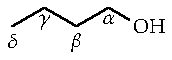
\includegraphics[width=3cm]{03-Butanol/nbuoh-skeletal}}%
                {\caption{\nBuOH{}}\label{fig:nbuoh-skeletal}}%
            \ffigbox
                {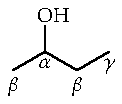
\includegraphics[width=3cm]{03-Butanol/sbuoh-skeletal}}%
                {\caption{\sBuOH{}}\label{fig:sbuoh-skeletal}}%
            \ffigbox
                {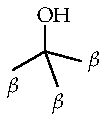
\includegraphics[height=2.5cm]{03-Butanol/tbuoh-skeletal}}%
                {\caption{\tBuOH{}}\label{fig:tbuoh-skeletal}}%
            \ffigbox
                {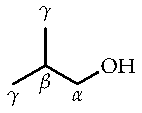
\includegraphics[width=3cm]{03-Butanol/ibuoh-skeletal}}%
                {\caption{\iBuOH{}}\label{fig:ibuoh-skeletal}}%
        \end{subfloatrow}
    }%
    {\caption{Skeletal structures of the butanol isomers}
    \label{fig:buoh-isomers}}
\end{figure}

\section{Structure of the Butanol Isomers}
\label{sec:butanol-isomers}

Butanol is the four carbon alcohol, and has four isomers:
\nBuOH{} (1-butanol);
\sBuOH{} (2-butanol);
\tBuOH{} (2-methyl-2-propanol); and
\iBuOH{} (2-methyl-1-propanol).
The skeletal structures of the four isomers are shown in
\cref{fig:buoh-isomers}. The carbon atoms in the skeleton are
labeled according to their distance from the hydroxyl moeity; the
$\alpha$ carbon is the closest to the hydroxyl, followed by $\beta$,
$\gamma$, and $\delta$ carbons. Not all of the butanols have all of
the types of carbons listed here, due to varying chain lengths. For
instance, \tBuOH{} has one $\alpha$ carbon (not labeled), three $\beta$
carbons, and no $\gamma$ or $\delta$ carbons.


Three of the butanol isomers can be produced
by biological pathways (\textit{n}-, \textit{s}-, and \iBuOH{})
\cite{Nigam2011,Smith2010}, making them candidates for the ``second-generation''
of biofuels \cite{Harvey2011,Nigam2011}. Although \tBuOH{} does not have
an identified biological production pathway, it has commercial significance
as an octane enhancer. In addition, the four isomers of butanol represent
the smallest alcohol system with all four types of branching in the skeleton.
This makes them excellent candidates to build kinetic models that can be
extended to larger alcohols with similar structures.

\Cref{tab:buoh-heats} shows a comparison of the higher heating value of
the butanol isomers with ethanol and gasoline. The higher energy density
of the butanol isomers allows them to be blended in gasoline in higher
proportions and reduces the volumetric fuel economy (e.g. mpg) impact
of replacing gasoline with biofuels.

\section{Experimental Procedure}
\label{sec:buoh-proc}

The reactants used in this study, along with their purities, are shown in
\cref{tab:buoh-expts}. To determine the relative proportions of each
reactant in the mixture, the absolute mass of fuel, the equivalence ratio
($\phi$), and the oxidizer ratio ($X_{O_2}:X_{\mathrm{inert}}$, where $X$
indicates mole fraction) are specified. \textit{s}- and \textit{i}-Butanol are
liquid at room temperature and have relatively low vapor pressure; therefore,
each is massed in a syringe to within \SI{0.01}{g} of the specified
value. \textit{t}-Butanol is solid at room temperature (melting point: \SI{25}{\celsius}),
and is melted before being handled in the same procedure as the other fuels.
The \SI{17}{\liter} mixing tank is vacuumed to an ultimate pressure less than \SI{5}{Torr} prior
to the injection of the liquid fuel through a septum. Proportions of O$_2$ and
N$_2$ are added manometrically at room temperature. The preheat temperature of
the RCM is set above the saturation point for each fuel to ensure complete
vaporization. A magnetic stirrer mixes the reactants. The temperature inside
the mixing tank is allowed to equilibrate for approximately \SI{1.5}{\hour}.

This approach to mixture preparation has been validated in several previous
studies by withdrawing gas samples from the mixing tank and analyzing the
contents by GC/MS \cite{Weber2011}, GC-FID \cite{Kumar2009}, and GC-TCD
\cite{Das2012}. These studies have verified the concentration of
\nBuOH{}, \textit{n}-decane, and water, respectively. In addition,
both the work by \textcite{Kumar2009} on \textit{n}-decane and the study of
\textcite{Weber2011} on \nBuOH{} confirmed that there was no fuel
decomposition over the course of a typical set of experiments. Furthermore,
within this study, each new mixture preparation is checked against previously
tested conditions to ensure reproducibility.

\Cref{tab:buoh-expts} shows the experimental conditions considered in this
study. The compressed pressure conditions have been chosen to match the
previous \nBuOH{} study \cite{Weber2011}, but also to provide data in
regions not covered extensively in previous work. In addition, the fuel loading
conditions have been chosen to complement previous work; the studies by
\textcite{Stranic2012} and \textcite{Moss2008} used relatively dilute mixtures,
so we have included higher fuel loading conditions. Furthermore, the compressed
temperature conditions we have studied ($T_C=\SIrange{715}{910}{\kelvin}$) have not been examined
in any other study, to our knowledge.

Each compressed pressure and temperature condition is repeated at least six
times to ensure repeatability. The mean and standard deviation of the ignition
delay for all runs at each condition are calculated. As an indication of
repeatability, the standard deviation is less than 10\% of the mean in every
case. Representative experimental pressure traces for simulations and
presentation are then chosen as the closest to the mean.

\begin{table}
    \caption{Experimental Conditions and Reactant Purities}
    \label{tab:buoh-expts}
    \begin{tabular}{*{7}{c}}
    \toprule
    \multicolumn{5}{c}{Reactant (Purity)} & \multirow{3}[0]{*}{\linebreakcell{Equivalence \\ Ratio \\ $\phi$}} & \multirow{3}[0]{*}{\linebreakcell{Compressed \\ Pressure \\ $P_C$ (bar)}} \\
    \cmidrule{1-5}
    \linebreakcell{\sBuOH{} \\ (99.99\%)} & \linebreakcell{\iBuOH{} \\ (99.99\%)} & \linebreakcell{\tBuOH{} \\ (99.99\%)} & \linebreakcell{O$_2$ \\ (99.999\%)} & \linebreakcell{N$_2$ \\ (99.995\%)} & & \\
    \cmidrule{1-5}
    \multicolumn{5}{c}{Mole Percentage}   & & \\
    \midrule
    3.38  &       &       & 20.30 & 76.32 & 1.0 & 15 \\
    3.38  &       &       & 20.30 & 76.32 & 1.0 & 30 \\
          & 3.38  &       & 20.30 & 76.32 & 1.0 & 15 \\
          & 3.38  &       & 20.30 & 76.32 & 1.0 & 30 \\
          &       & 3.38  & 20.30 & 76.32 & 1.0 & 15 \\
          &       & 3.38  & 20.30 & 76.32 & 1.0 & 30 \\
          &       & 1.72  & 20.65 & 77.63 & 0.5 & 30 \\
          &       & 6.54  & 19.63 & 73.83 & 2.0 & 30 \\
    \bottomrule
    \end{tabular}
\end{table}

\section{Experimental Results}
\label{sec:buoh-expts}

\Cref{fig:buoh-15bar} shows the ignition delays of the four isomers of
butanol measured in the RCM, at compressed pressure of $P_C=\SI{15}{\bar}$ for
stoichiometric mixture in air. The dashed line for each isomer is a least
squares fit to the data. The vertical error bars are two standard deviations
of the measurements of the ignition delay. The standard deviation is computed
based on all the runs at a particular compressed temperature and pressure
condition. A conservative estimate of the uncertainty in $T_C$ was calculated
in our previous work to be approximately \SIrange{0.7}{1.7}{\percent}. Due to the similar nature
of these experiments, and the similar properties of the fuels, this estimate
is considered to be valid for this study as well.

\Cref{fig:buoh-15bar} demonstrates the differences in reactivity between
the isomers for stoichiometric fuel/air mixtures at compressed pressure
$P_C=\SI{15}{\bar}$. \textit{n}-Butanol is clearly the most reactive, followed by
\textit{s}- and \iBuOH{}, which have very similar reactivities in
this temperature and pressure range. \textit{t}-Butanol is the least reactive.

The order of reactivity found in the RCM at \SI{15}{\bar} agrees with the ST
study at higher temperatures (approximately \SIrange{1275}{1667}{\kelvin}) and lower pressure
(\SI{1.5}{atm}) by \textcite{Stranic2012} but differs slightly from the studies of
\textcite{Moss2008} who measured ignition delays in a ST near \SI{1.5}{atm}
and between \SIrange{1275}{1400}{\kelvin}, and \textcite{Veloo2011a} who measured
atmospheric-pressure laminar flame speeds. In particular, \textcite{Moss2008}
and \textcite{Veloo2011a} found distinct differences in reactivity between
\textit{s}- and \iBuOH{}, but the present study and the study by
\textcite{Stranic2012} found that they were nearly indistinguishable in terms
of reactivity under the conditions investigated. In addition,
\textcite{Stranic2012} noted some disagreement between their ST
ignition data and the data of \textcite{Moss2008} but their attempts to isolate
the cause could not discern what the difference might be caused by.

Further, the order of the reactivity of the butanol isomers shows complex
temperature and pressure dependence. This is demonstrated by the results shown
in \cref{fig:buoh-30bar}. In \cref{fig:buoh-30bar}, the order of
reactivity is different than in \cref{fig:buoh-15bar}, where the only
variation between the plots is the compressed pressure; in
\cref{fig:buoh-30bar} the compressed pressure is $P_C=\SI{30}{\bar}$.
\cref{fig:buoh-30bar} shows \iBuOH{} to be the least reactive,
\sBuOH{} to be less reactive than but similar to \tBuOH{},
and \nBuOH{} to be the most reactive. Interestingly, the results of
the ST study by \textcite{Stranic2012} differ from those in the current
study at higher pressure, despite the agreement at lower pressure. In their
study, \textcite{Stranic2012} found \textit{i}- and \nBuOH{} to have
similar reactivity near \SI{43}{atm} in the temperature range of \SIrange{1020}{1280}{\kelvin},
whereas in the present study we find \iBuOH{} to be the least
reactive of all four isomers at a pressure of \SI{30}{\bar} and over the temperature
range (\SIrange{715}{910}{\kelvin}) investigated.

\begin{figure}
    \begin{floatrow}
    \ffigbox
        {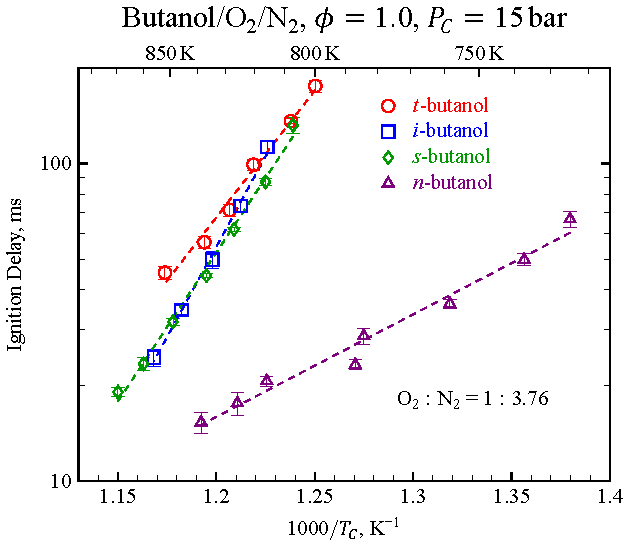
\includegraphics[width=7.9cm]{03-Butanol/buoh-15bar}}
        {\caption{Ignition delays of the four isomers of butanol at compressed
            pressure $P_C=\SI{15}{\bar}$. Dashed lines are least squares fits to the
            data.}
        \label{fig:buoh-15bar}}
    \ffigbox
        {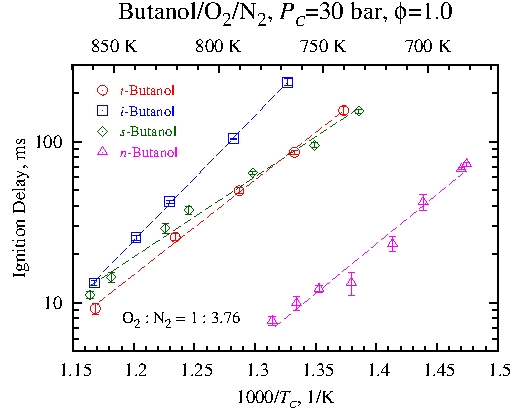
\includegraphics[width=7.9cm]{03-Butanol/buoh-30bar}}
        {\caption{Ignition delays of the four isomers of butanol at compressed
            pressure $P_C=\SI{30}{\bar}$. Dashed lines are least squares fits to the
            data.}
        \label{fig:buoh-30bar}}
    \end{floatrow}
\end{figure}

The fact that \tBuOH{} becomes relatively more reactive than
\textit{i}- and \sBuOH{} as pressure increases is surprising at first
glance, and the reasons are not immediately apparent. Closer examination of the
pressure traces for each experiment gives one clue as to the cause of the
increased reactivity. \Cref{fig:tbuoh-15bar} shows the pressure traces for
the \tBuOH{} experiments at \SI{15}{\bar} for stoichiometric mixtures in
air. It is evident that there is some pre-ignition heat release, because the
reactive pressure trace diverges from the non-reactive case prior to the
ignition event. Of the other isomers of butanol, only \nBuOH{} shows
any visible heat release prior to the main ignition event at \SI{15}{\bar}.

\Cref{fig:tbuoh-phi10} shows the pressure traces for \tBuOH{}
experiments at \SI{30}{\bar} for stoichiometric mixtures in air. The effect of
pre-ignition heat release is even more striking in this figure, with
substantial changes in the slope of the pressure trace during the reactive
runs. Comparison to the pressure traces of the other isomers once again shows
that the magnitude of the pre-ignition heat release for \tBuOH{} is
much greater. Despite the appearance of early pressure rise, which is typically
indicative of two-stage ignition and low temperature chain branching, we do not
find a negative temperature coefficient region in terms of the ignition delay
response for any \tBuOH{} experiments. Therefore, we adopt the phrase
``pre-ignition heat release'' rather than ``two-stage ignition'' in this work.

\begin{figure}
    \begin{floatrow}
    \ffigbox
        {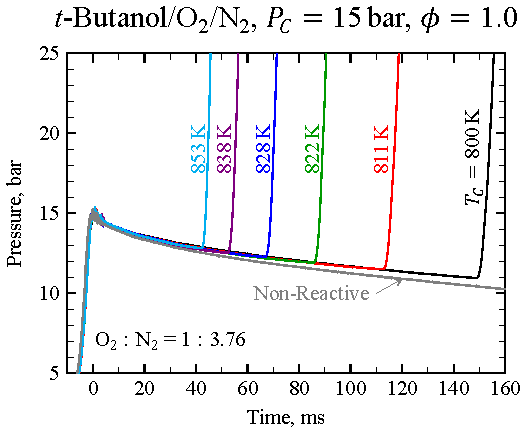
\includegraphics[width=7.9cm]{03-Butanol/tbuoh-15bar}}
        {\caption{Pressure traces of the \SI{15}{\bar} \tBuOH{} experiments,
            in stoichiometric air.}
        \label{fig:tbuoh-15bar}}
    \ffigbox
        {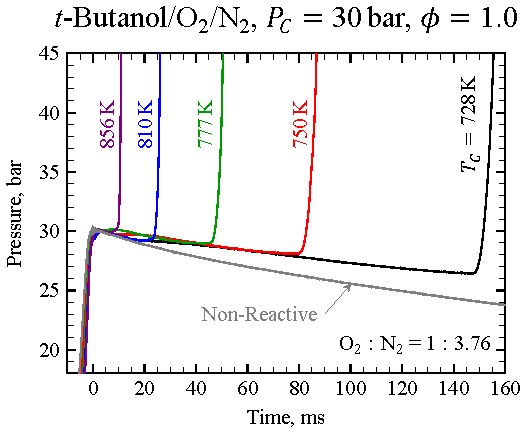
\includegraphics[width=7.9cm]{03-Butanol/tbuoh-phi10}}
        {\caption{Pressure traces of the \SI{30}{\bar} \tBuOH{} experiments,
            in stoichiometric air.}
        \label{fig:tbuoh-phi10}}
    \end{floatrow}
\end{figure}

In an effort to understand the reactions causing the pre-ignition heat release,
further experiments are conducted for \tBuOH{} at $P_C=\SI{30}{\bar}$, for
equivalence ratios of 0.5 and 2.0 in air. \Cref{fig:tbuoh-delays} shows
Arrhenius plots of the ignition delays for the three equivalence ratios. As
with the previous \nBuOH{} experiments at \SI{15}{\bar} \cite{Weber2011}
$\phi=\num{0.5}$ is the least reactive and $\phi=\num{2.0}$ is the most reactive. The
slopes are similar, indicating that the overall activation energies are similar
for the conditions investigated.

\begin{figure}
    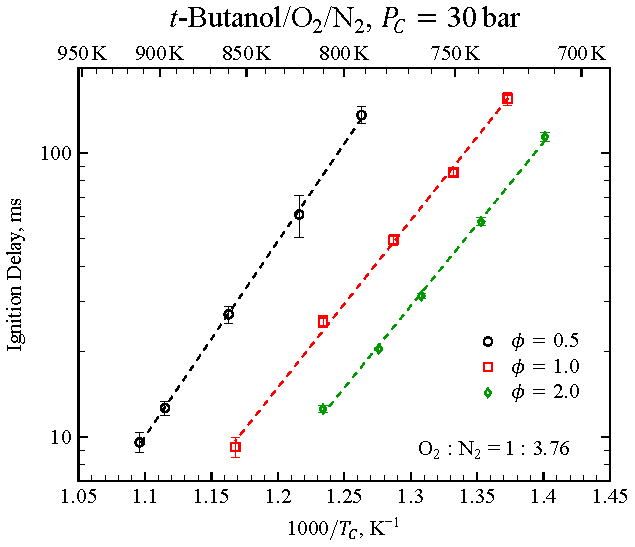
\includegraphics[width=12cm]{03-Butanol/tbuoh-delays}
    \caption{Ignition delays of three equivalence ratios of \tBuOH{}
    in air, for $P_C=\SI{30}{\bar}$. Lines represent least squares fits to the data.}
    \label{fig:tbuoh-delays}
\end{figure}

A more interesting comparison is of the pressure traces of the three
equivalence ratios. It is clear from \cref{fig:tbuoh-phi10,fig:tbuoh-phi05,%
fig:tbuoh-phi20} that there are qualitative differences in the pre-ignition
heat release between the three equivalence ratios. This is most likely
due to the effect of the increased (reduced) fuel mole fraction in the
$\phi=\num{2.0}$ ($\phi=\num{0.5}$) case, since the mole fraction of
fuel is changed by +93\% (-49\%) compared to the $\phi=\num{1.0}$ case, while the
mole fraction of oxygen changes by only -3\% (+2\%) compared to the $\phi=\num{1.0}$
case, as shown in \cref{tab:buoh-expts}. Therefore, it appears that the
qualitative change in pre-ignition behavior is due to the change of fuel mole
fraction, where higher fuel loading promotes pre-ignition heat release.

\begin{figure}
    \begin{floatrow}
    \ffigbox
        {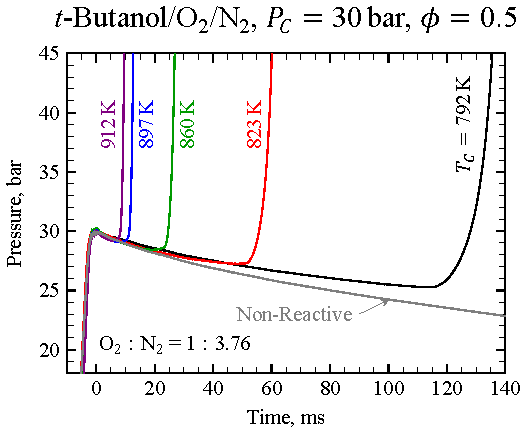
\includegraphics[width=7.9cm]{03-Butanol/tbuoh-phi05}}
        {\caption{Pressure traces of the \SI{30}{\bar} \tBuOH{} experiments,
            $\phi=\num{0.5}$ in air.}
        \label{fig:tbuoh-phi05}}
    \ffigbox
        {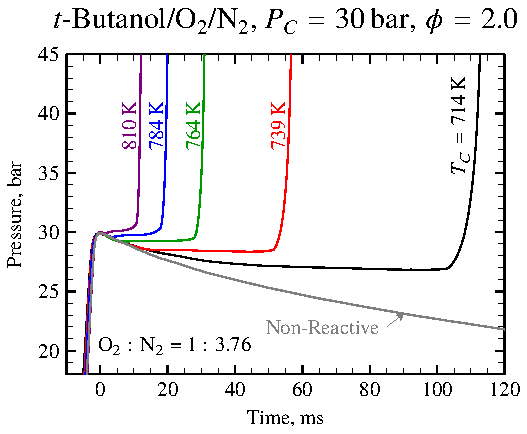
\includegraphics[width=7.9cm]{03-Butanol/tbuoh-phi20}}
        {\caption{Pressure traces of the \SI{30}{\bar} \tBuOH{} experiments,
            $\phi=\num{2.0}$ in air.}
        \label{fig:tbuoh-phi20}}
    \end{floatrow}
\end{figure}

\section{Simulation Results}
\label{sec:buoh-sims}

Simulations are performed with the kinetic mechanism from
\textcite{Sarathy2012} denoted as the Sarathy et al. mechanism, and a
recent mechanism discussed by \textcite{Hansen2013} and
\textcite{Merchant2013} that is denoted as the MIT mechanism hereafter.
Other recent mechanisms, such as the mechanism from
\textcite{Frassoldati2012} do not include low temperature chemistry and are
therefore unable to reproduce the low-temperature ignition delays measured in
this study. The study by \textcite{Sarathy2012} validated their model for a
wide set of the existing experimental data. In terms of ignition delays, this
included the data from the study of \textcite{Stranic2012} up to \SI{48}{atm}, our
previous study on \nBuOH{} \cite{Weber2011}, and the data being
published in this study at \SI{15}{\bar}. Importantly, the mechanism of
\textcite{Sarathy2012} was validated only for the \SI{15}{\bar} RCM data for all four
isomers, but not the \SI{30}{\bar} data also being published here. The MIT mechanism
\cite{Hansen2013,Merchant2013} was validated for \iBuOH{}
experiments, including pyrolysis and low pressure premixed flames; although the
model includes all four isomers of butanol as reactants, it has not been
optimized for any of the isomers except \iBuOH{}.

\Cref{fig:buoh-15sim,fig:buoh-30sim} show comparison of the
VPRO simulations with the experimental data using the mechanism of
\textcite{Sarathy2012}. As \textcite{Sarathy2012} showed in their work (and as
we show here in \cref{fig:buoh-15sim}), they found good agreement of the
model predictions with the present RCM data at \SI{15}{\bar}. At $P_C=\SI{30}{\bar}$
(\cref{fig:buoh-30sim}), similar degree of agreement is found for
\tBuOH{} and \sBuOH{} compared to $P_C=\SI{15}{\bar}$, although
the \sBuOH{} results are under-predicted at high temperature and
over-predicted at low temperature. While the model of \textcite{Sarathy2012} is
able to well capture the overall activation energy of \iBuOH{}, it
under-predicts the experimental data by about a factor of \numrange{2}{3}. The
\nBuOH{} data are over-predicted by a factor of about 1.5.
Nevertheless, this agreement is quite good, especially considering that the
model is not validated for these conditions.

\begin{figure}
    \begin{floatrow}
    \ffigbox
        {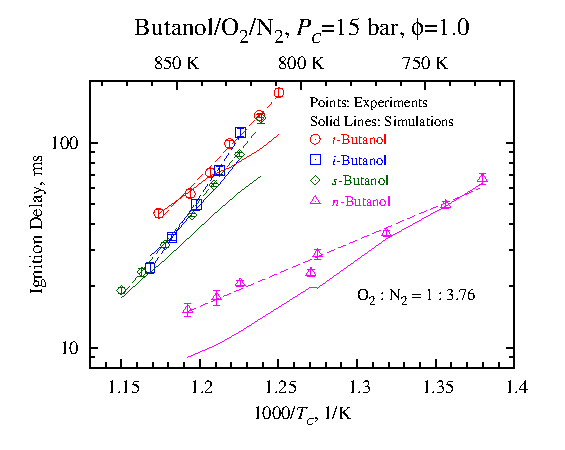
\includegraphics[width=7.9cm]{03-Butanol/buoh-15sim}}
        {\caption{$P_C=\SI{15}{\bar}$, stoichiometric mixtures in air. Comparison of
            VPRO simulations using the kinetic mechanism of
            \textcite{Sarathy2012} with experimental ignition delays.}
        \label{fig:buoh-15sim}}
    \ffigbox
        {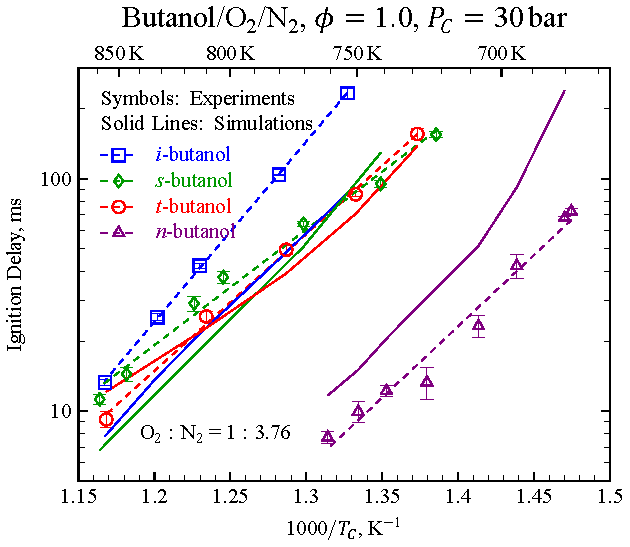
\includegraphics[width=7.9cm]{03-Butanol/buoh-30sim}}
        {\caption{$P_C=\SI{30}{\bar}$, stoichiometric mixtures in air. Comparison of
            VPRO simulations using the kinetic mechanism of
            \textcite{Sarathy2012} with experimental ignition delays.}
        \label{fig:buoh-30sim}}
    \end{floatrow}
\end{figure}

VPRO simulations for \textit{n}- and \sBuOH{} (and also \tBuOH{} under
some conditions) using the MIT mechanism
\cite{Hansen2013,Merchant2013} do not ignite during the duration of the
simulations (the same as the experimental duration), and therefore no
simulations are shown for these fuels. In \cref{fig:buoh-mit}, VPRO
simulations at \SIlist{15;30}{\bar} using both mechanisms are shown for
\iBuOH{}. The mechanism from \textcite{Sarathy2012}
is in better agreement at \SI{15}{\bar}. However, at \SI{30}{\bar} the MIT mechanism
\cite{Hansen2013,Merchant2013} over-predicts the ignition delay (as at \SI{15}{\bar}),
while the \textcite{Sarathy2012} mechanism under-predicts the ignition delay.
The reason for these diverging predictions will be explored and discussed below.

The agreement of the mechanism by \textcite{Sarathy2012} with the
off-stoichiometric mixtures of \tBuOH{} is also quite good, as shown
in \cref{fig:tbuoh-sims}. \Cref{fig:tbuoh-05press,fig:tbuoh-10press,,%The double comma is necessary to prevent compression
fig:tbuoh-20press} show more detailed comparisons
of the simulated pressure traces and the experimental results, for similar
temperatures at the three equivalence ratios, respectively. Clearly, the
simulations also exhibit some pre-ignition heat release. In general, the
simulations qualitatively predict the pre-ignition heat release behavior at all
three equivalence ratios. The $\phi=\num{0.5}$ case has the least heat release and
the $\phi=\num{2.0}$ case has the most. Although the simulations are unable to match
the heat release behavior quantitatively, they match the experimental ignition
delays quite well. Considering the model is not validated for this temperature,
pressure, and equivalence ratio regime, the mismatch of the pre-ignition
behavior may not be of critical importance, depending on the application.

\begin{figure}
    \begin{floatrow}
        \ffigbox
            {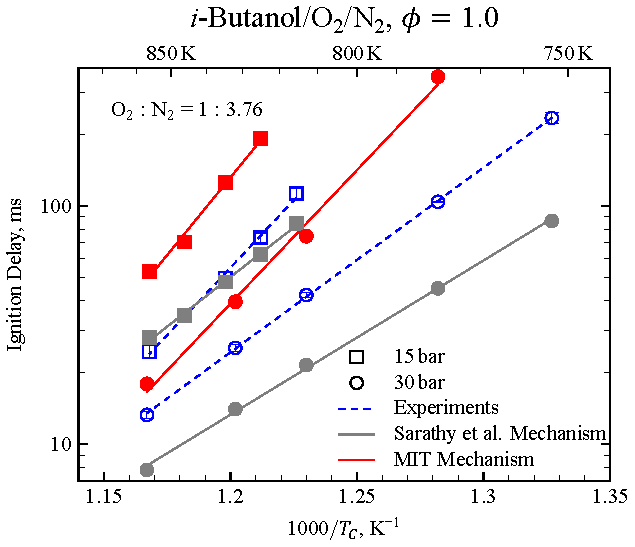
\includegraphics[width=7.9cm]{03-Butanol/buoh-mit}}
            {\caption{Comparison of VPRO simulations using the kinetic mechanism of
                \textcite{Sarathy2012} (solid lines) and the MIT mechanism
                \cite{Hansen2013,Merchant2013} (dotted lines) with the experimental
                ignition delay results (dashed lines) for stoichiometric mixtures of
                \iBuOH{} in air at $P_C=\SI{15}{\bar}$ (squares) and $P_C=\SI{30}{\bar}$
                (circles).}
            \label{fig:buoh-mit}}
        \ffigbox
            {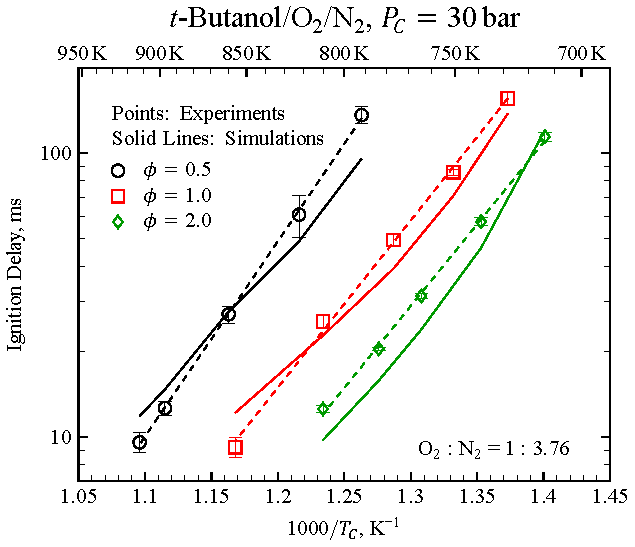
\includegraphics[width=7.9cm]{03-Butanol/tbuoh-sims}}
            {\caption{Comparison of the simulations using the kinetic mechanism of
                \textcite{Sarathy2012} for three equivalence ratio mixtures of
                \tBuOH{} in air at $P_C=\SI{30}{\bar}$.}
            \label{fig:tbuoh-sims}}
    \end{floatrow}
\end{figure}

\begin{figure}
    \ffigbox{%
    \begin{subfloatrow}[3]
        \ffigbox[\FBwidth]
            {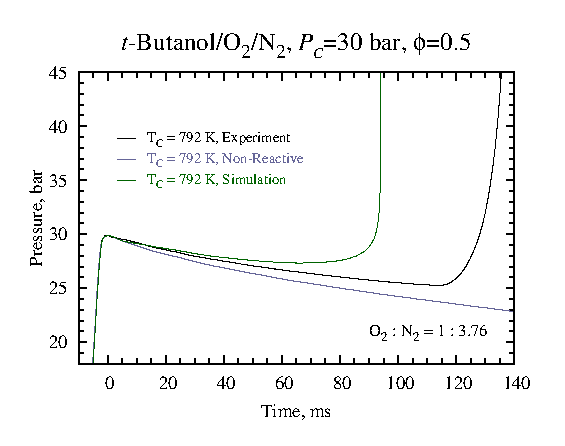
\includegraphics[width=5.2cm]{03-Butanol/tbuoh-05press}}
            {\caption{$\phi=\num{0.5}$ in air.}
            \label{fig:tbuoh-05press}}
        \ffigbox[\FBwidth]
            {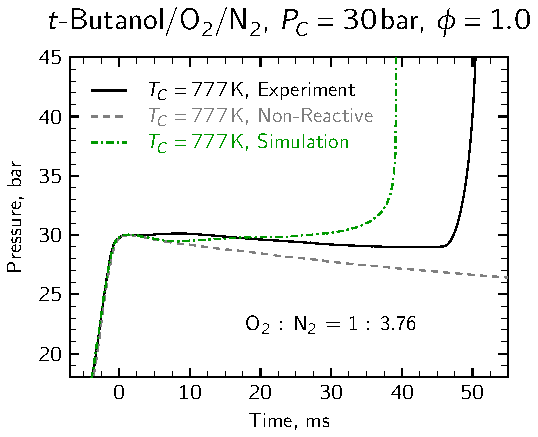
\includegraphics[width=5.2cm]{03-Butanol/tbuoh-10press}}
            {\caption{$\phi=\num{1.0}$ in air.}
            \label{fig:tbuoh-10press}}
        \ffigbox[\FBwidth]
            {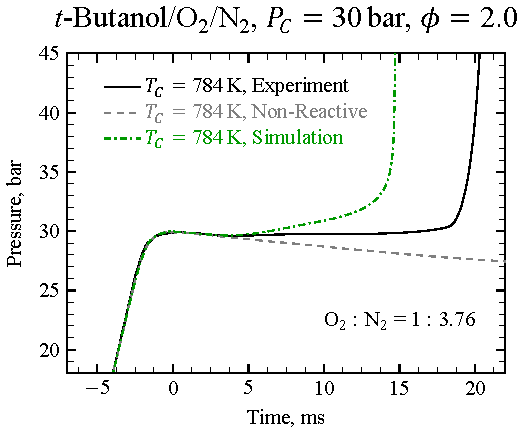
\includegraphics[width=5.2cm]{03-Butanol/tbuoh-20press}}
            {\caption{$\phi=\num{2.0}$ in air.}
            \label{fig:tbuoh-20press}}
    \end{subfloatrow}
    }%
    {\caption{Pressure traces of selected
     \tBuOH{} experiments compared with the corresponding
     non-reactive and simulated traces, using the mechanism of
     \textcite{Sarathy2012}.}
    }
\end{figure}

\section{Discussion}
\label{sec:buoh-discussion}

The relatively good agreement of the mechanism of \textcite{Sarathy2012} with
the experimental data, even for conditions at which the mechanism has not been
validated, suggests that using the mechanism to further interpret our
experimental data is a worthwhile exercise. In particular,
\cref{fig:buoh-npath,fig:buoh-spath,fig:buoh-tpath,fig:buoh-ipath}
show the initial steps of the fuel breakdown process for each isomer.
The percentages listed are the percent of the reactant that is consumed
to produce the product shown, by all the reactions that can produce
that product from the reactant, except where one particular reaction
is noted. These numbers are determined by integrating the
rate of production or consumption of each species by each reaction up to the
point of 20\% fuel consumption, and normalizing each reaction by the total
produced or consumed of each species up to that point. The 20\% fuel
consumption point is chosen because it is before small molecule chemistry takes
over to drive the ignition, and it has been used previously
\cite{Weber2011,Sarathy2012}. The rates of production are taken from a CONV
simulation, with initial conditions of \SI{750}{\kelvin} and \SI{15}{\bar} as well as \SI{750}{\kelvin} and
\SI{30}{\bar}. These conditions are representative of typical conditions after compression
in the present RCM experiments. The plain text percentages on top of the arrows
are the \SI{15}{\bar} case and the bold numbers underneath are for the \SI{30}{\bar} case.

\begin{figure}
    \begin{floatrow}
    \ffigbox
        {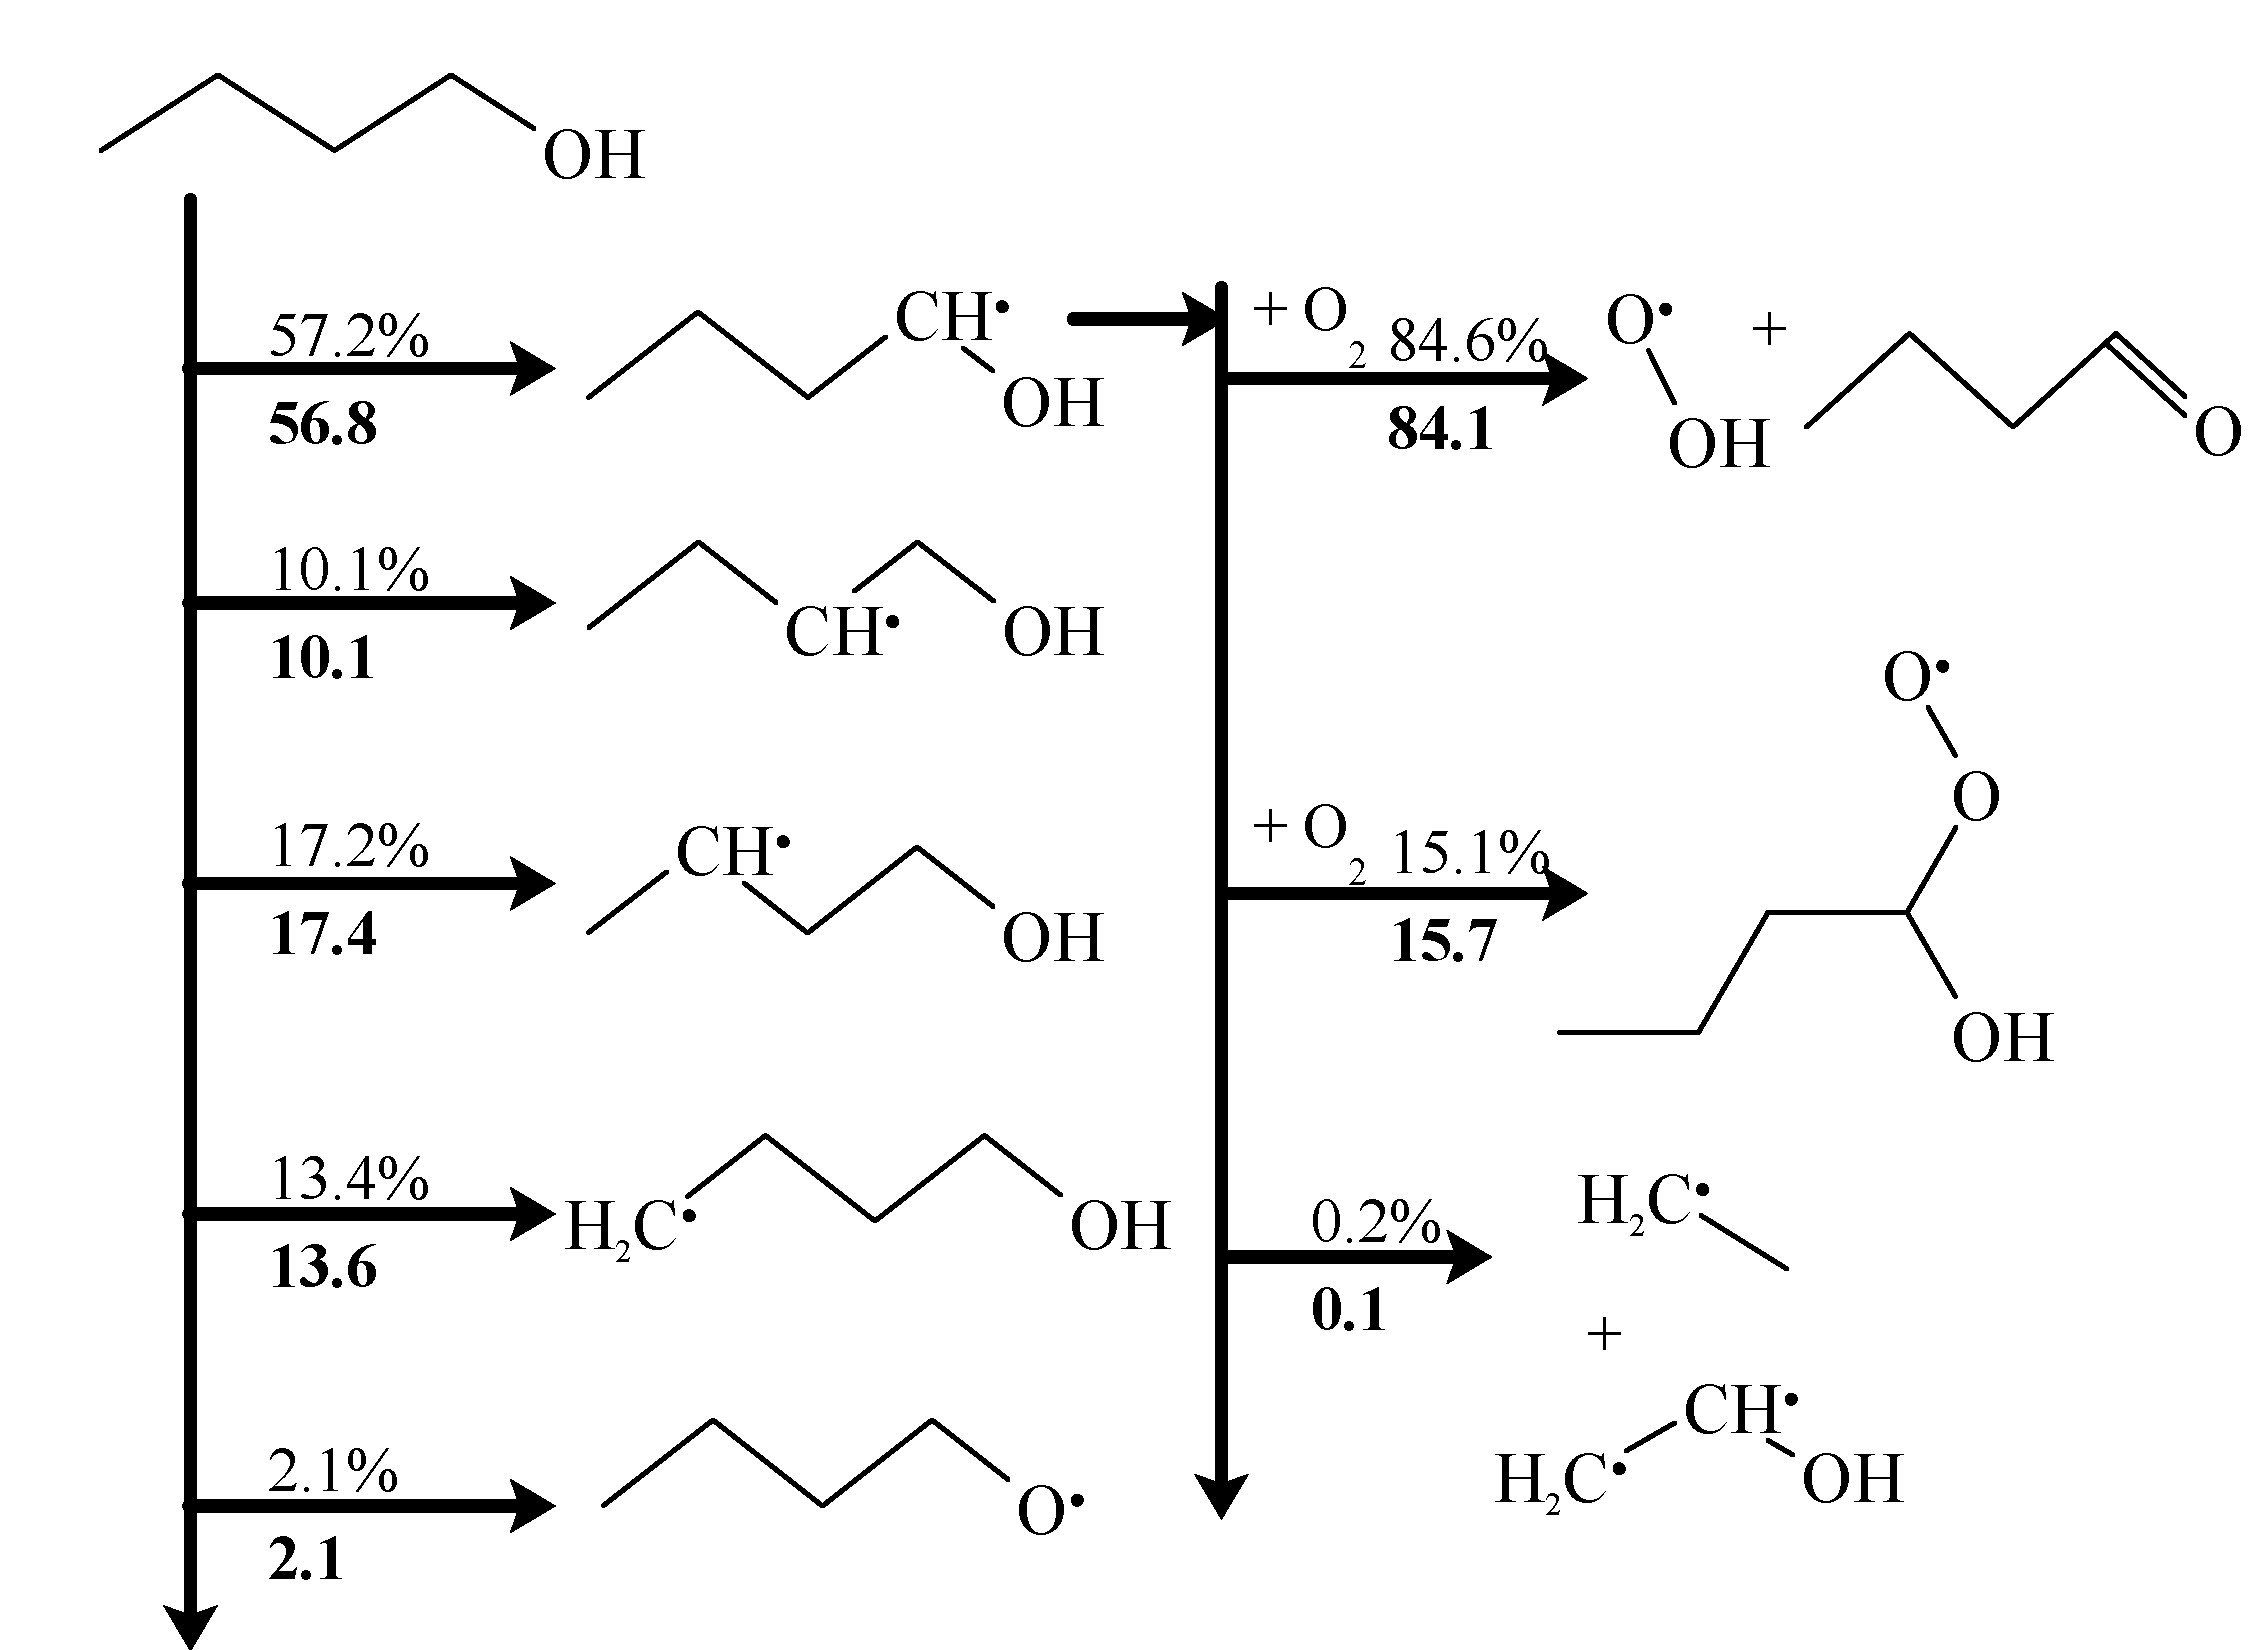
\includegraphics[width=7.9cm]{03-Butanol/buoh-npath}}
        {\caption{Pathway analysis for simulations of \nBuOH{} at
            temperature of \SI{750}{\kelvin}, in stoichiometric air, using the mechanism of
            \textcite{Sarathy2012}. Percentages in normal text represent an
            initial condition of \SI{15}{\bar}; bold text is for \SI{30}{\bar}.}
        \label{fig:buoh-npath}}
    \ffigbox
        {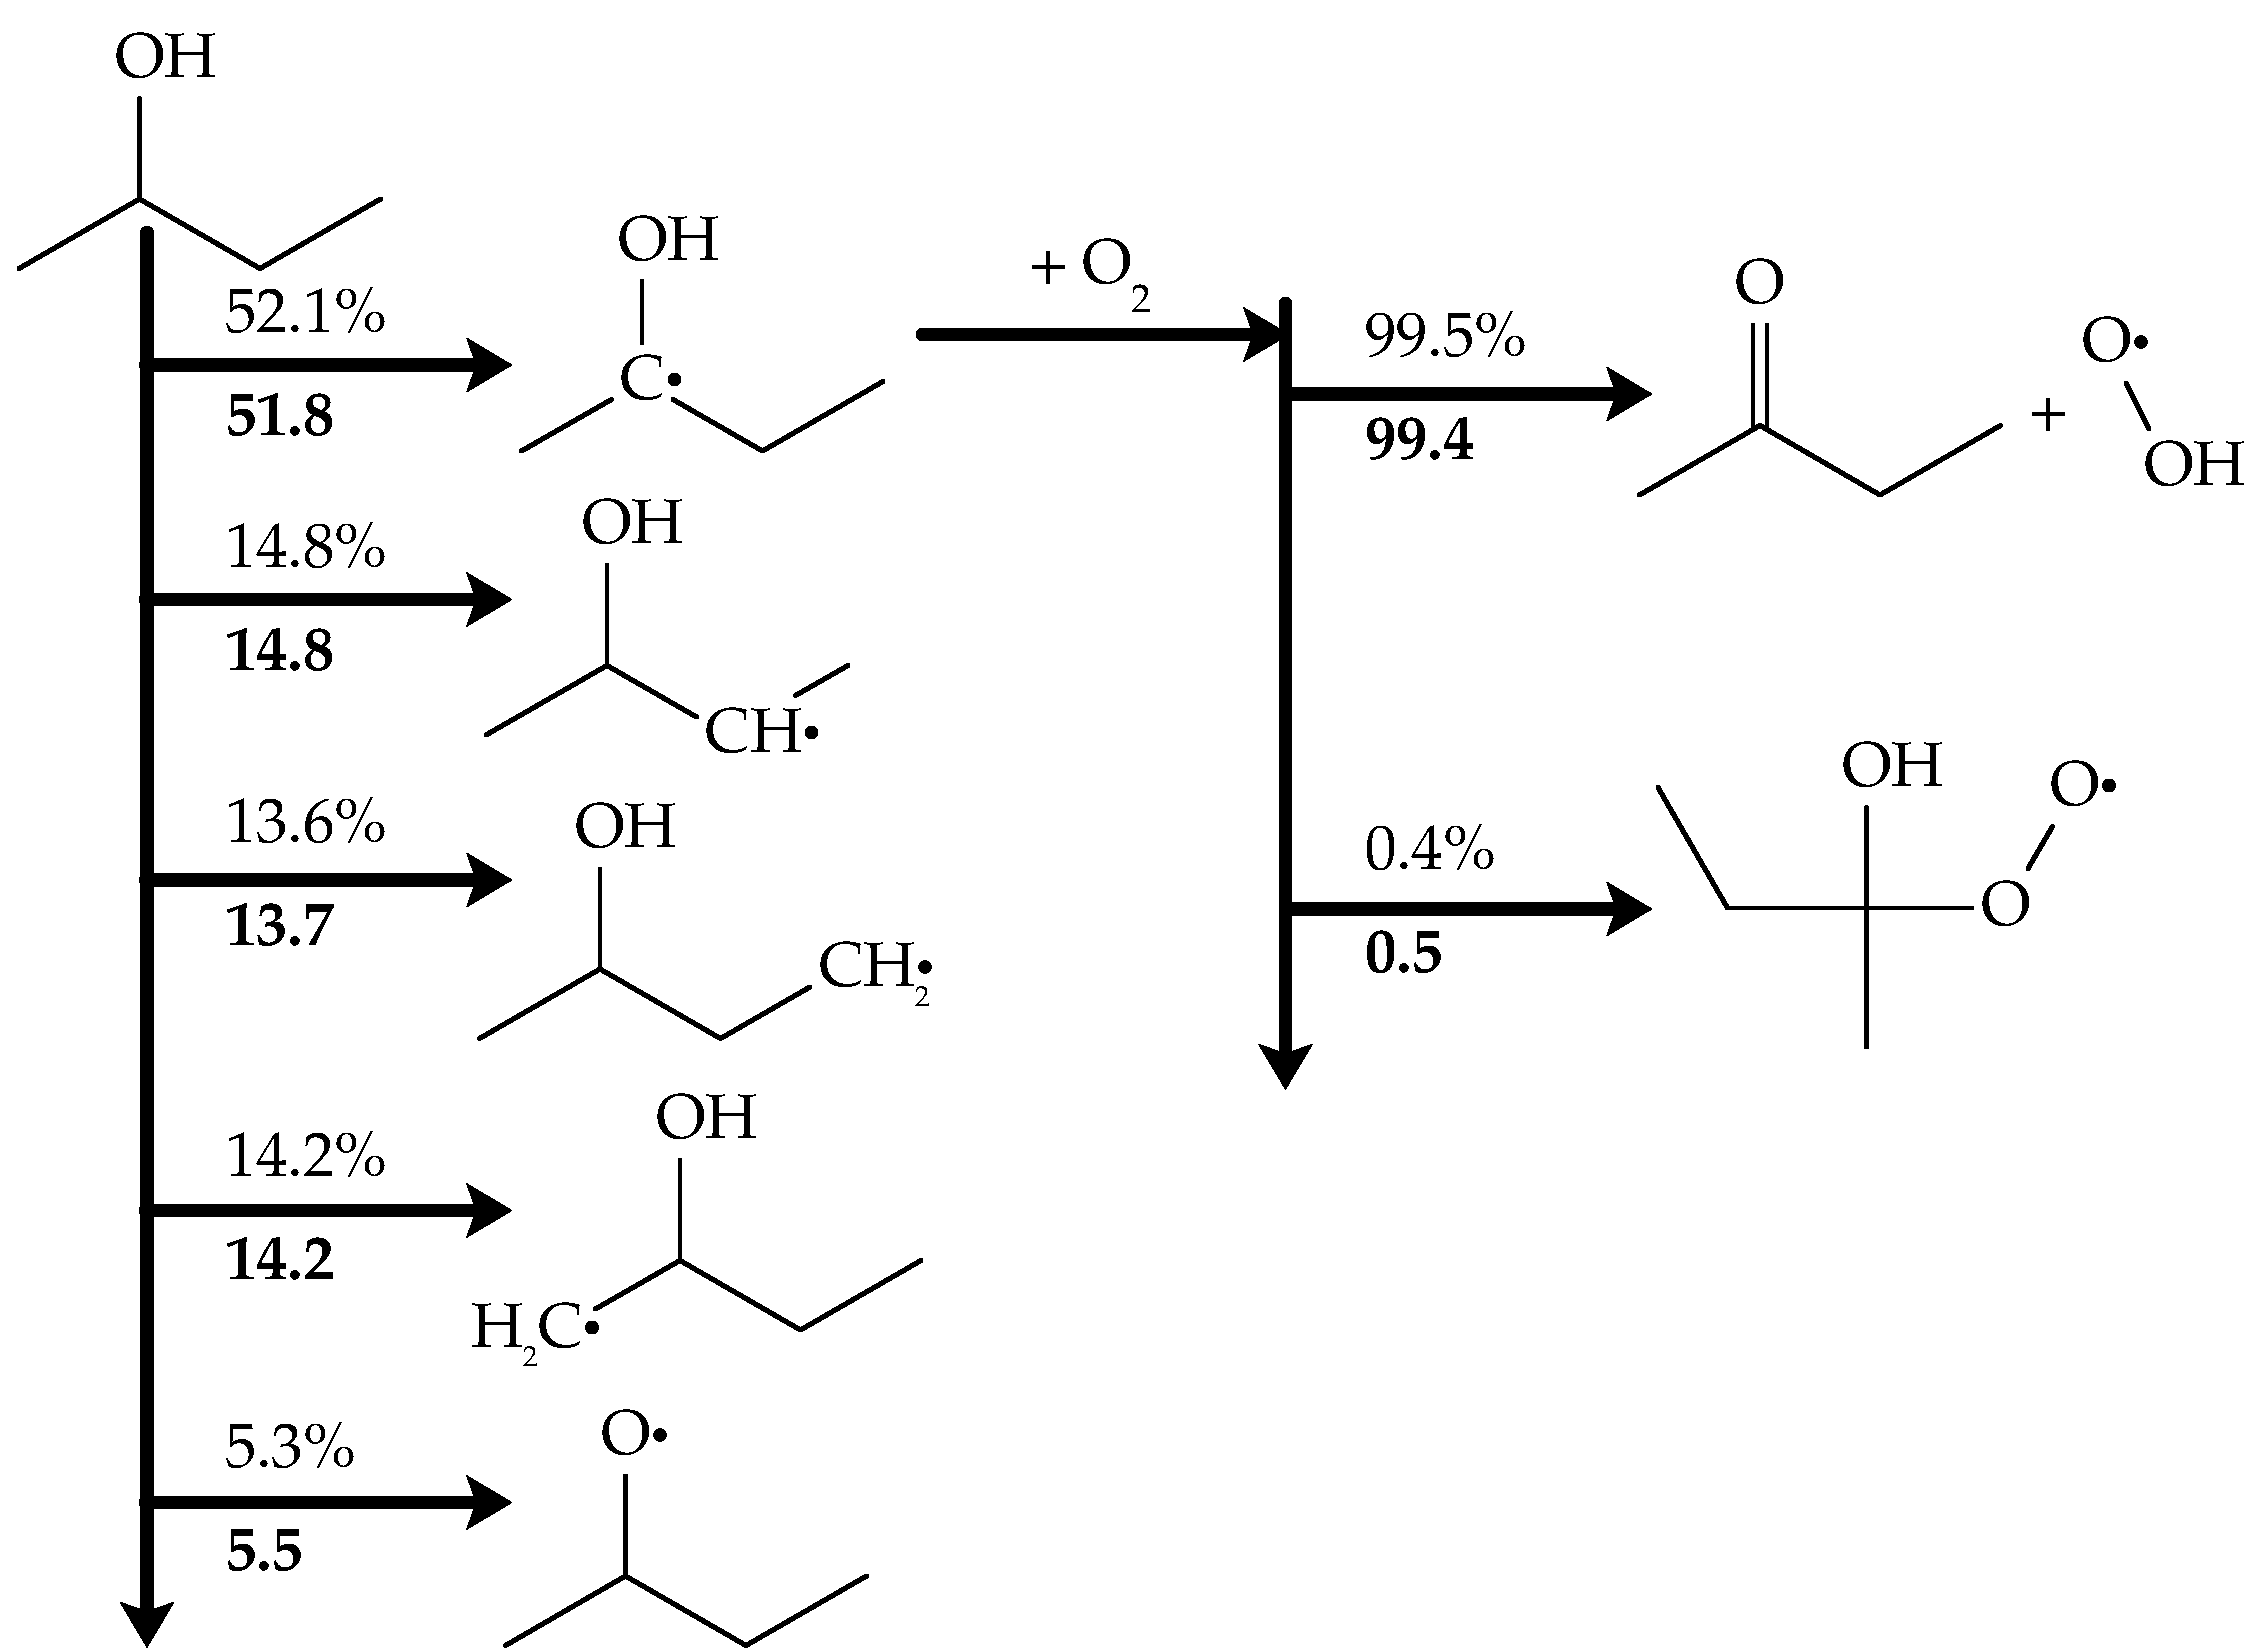
\includegraphics[width=7.9cm]{03-Butanol/buoh-spath}}
        {\caption{Pathway analysis for simulations of \sBuOH{} at
            temperature of \SI{750}{\kelvin}, in stoichiometric air, using the mechanism of
            \textcite{Sarathy2012}. Percentages in normal text represent an
            initial condition of \SI{15}{\bar}; bold text is for \SI{30}{\bar}.}
        \label{fig:buoh-spath}}
    \end{floatrow}
    \par
    \begin{floatrow}
    \ffigbox
        {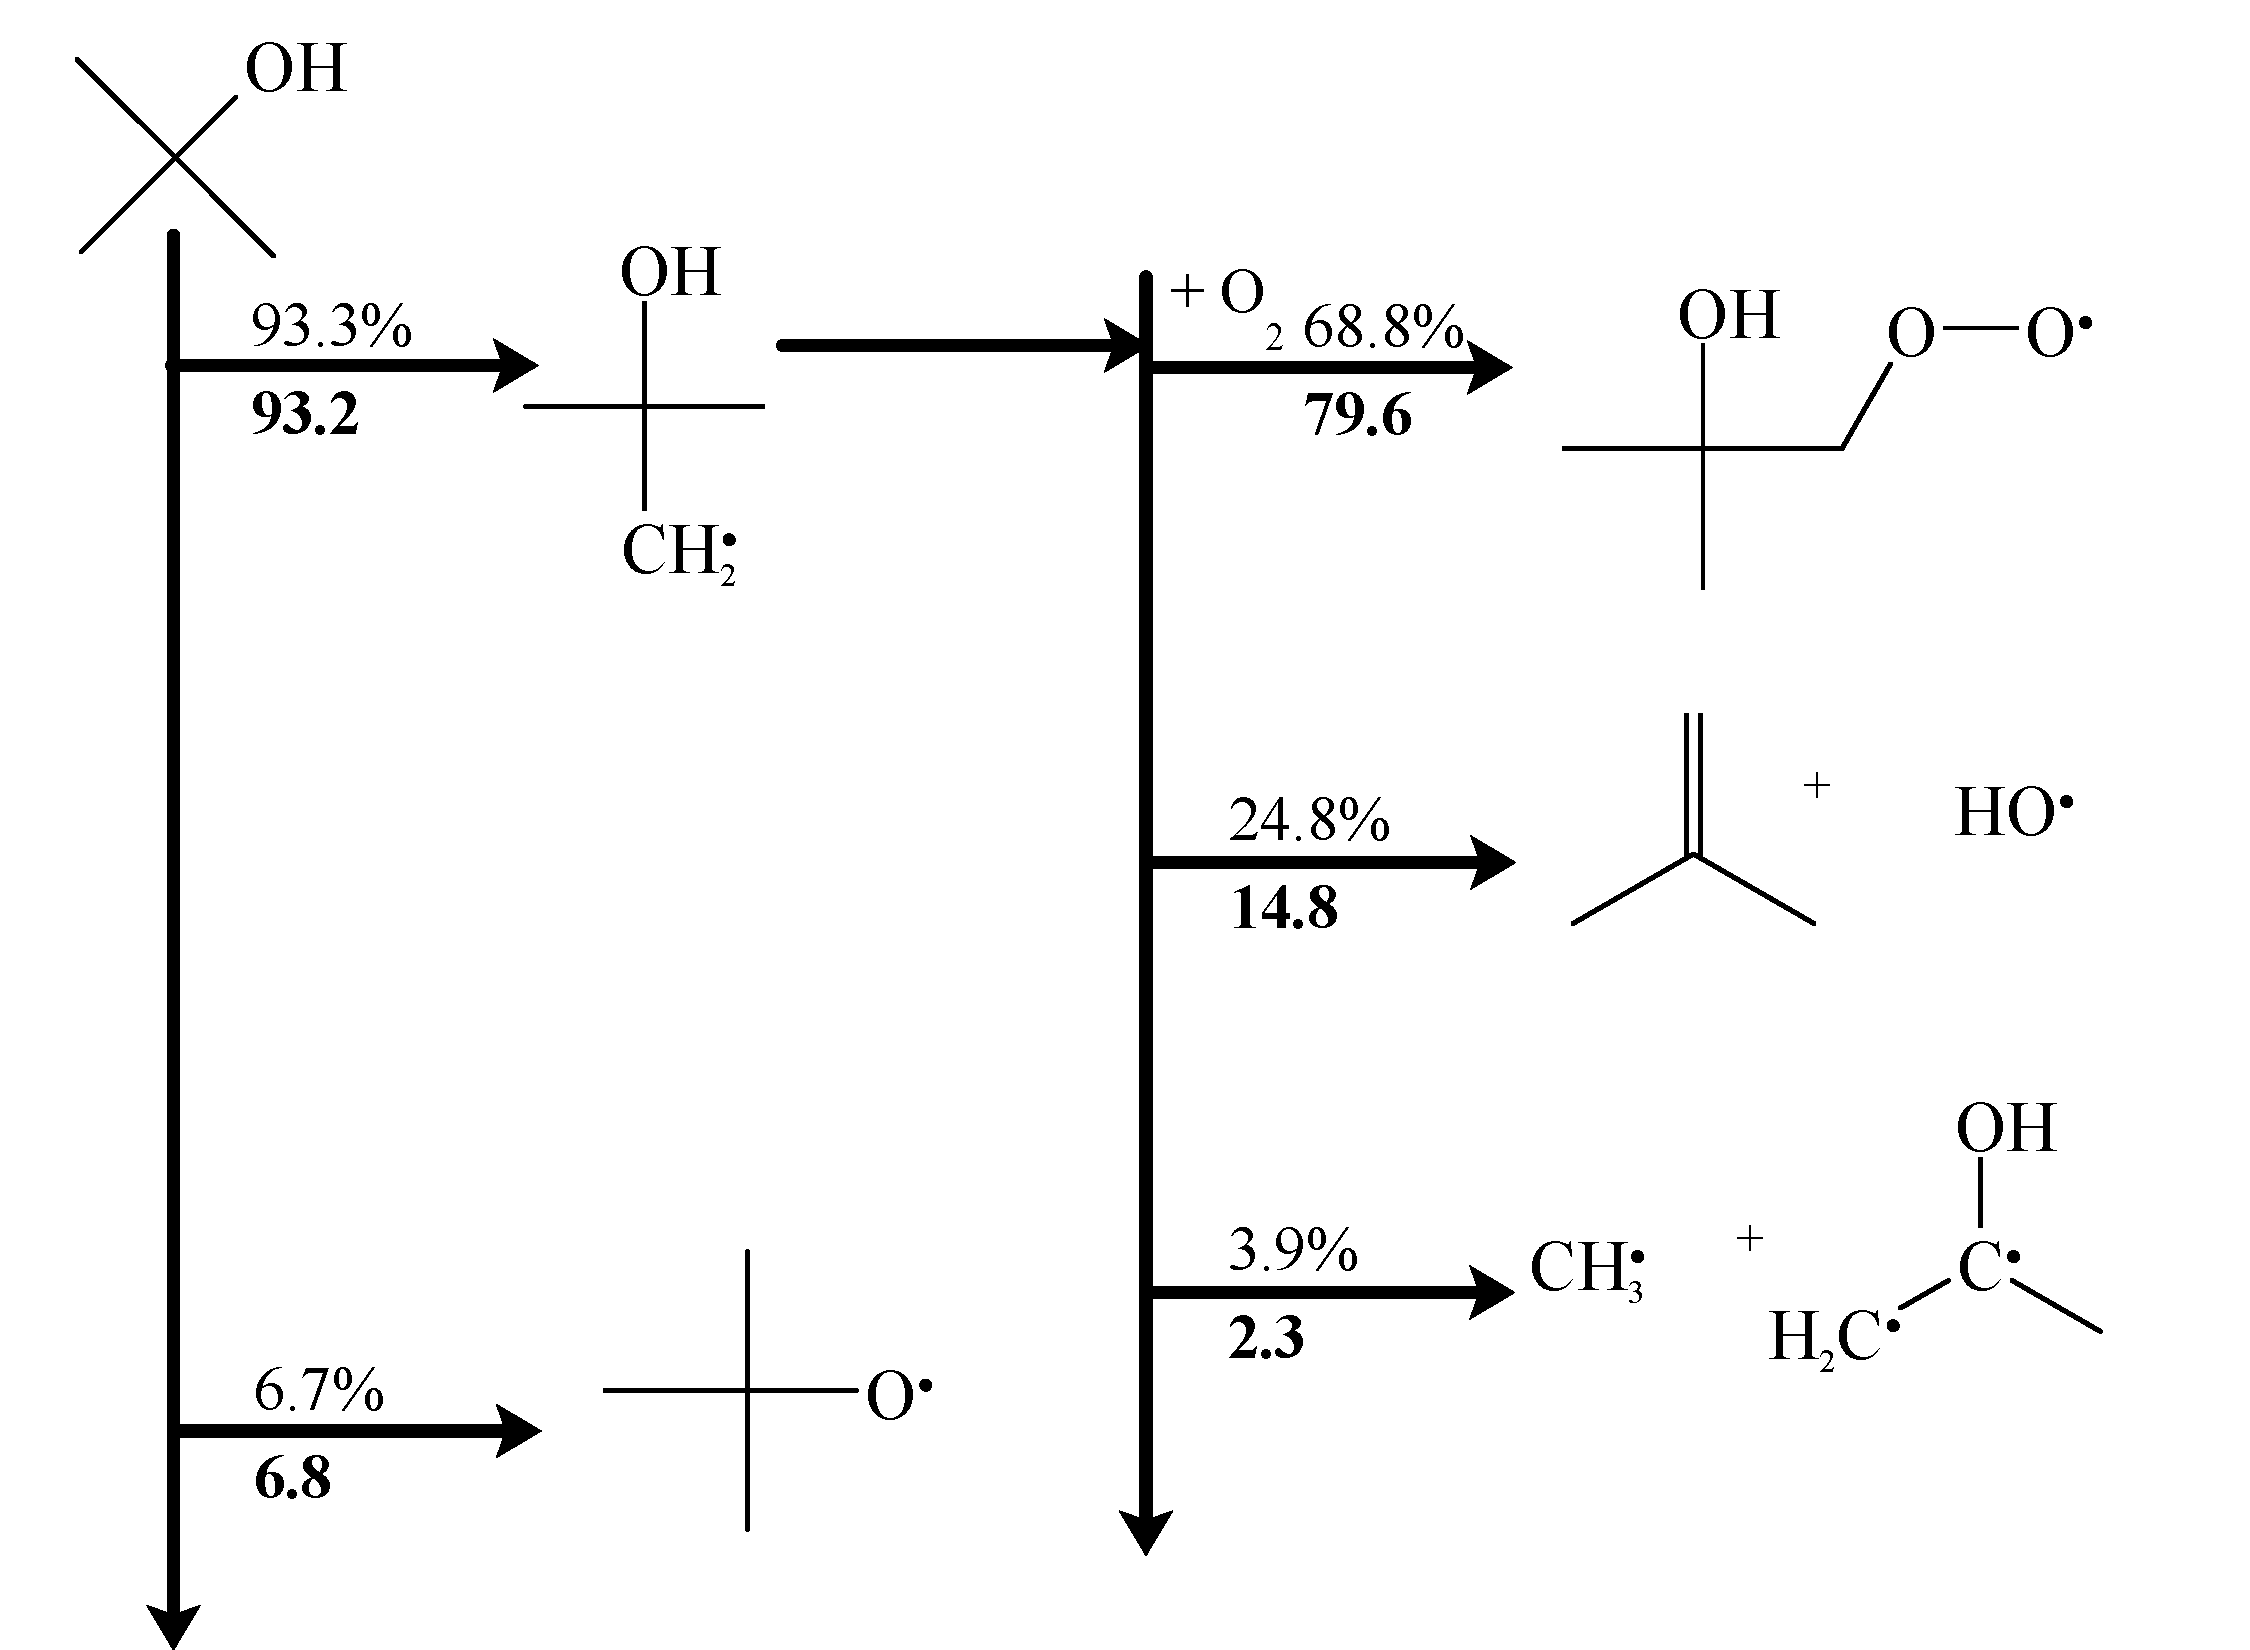
\includegraphics[width=7.9cm]{03-Butanol/buoh-tpath}}
        {\caption{Pathway analysis for simulations of \tBuOH{} at
            temperature of \SI{750}{\kelvin}, in stoichiometric air, using the mechanism of
            \textcite{Sarathy2012}. Percentages in normal text represent an
            initial condition of \SI{15}{\bar}; bold text is for \SI{30}{\bar}.}
        \label{fig:buoh-tpath}}
    \ffigbox
        {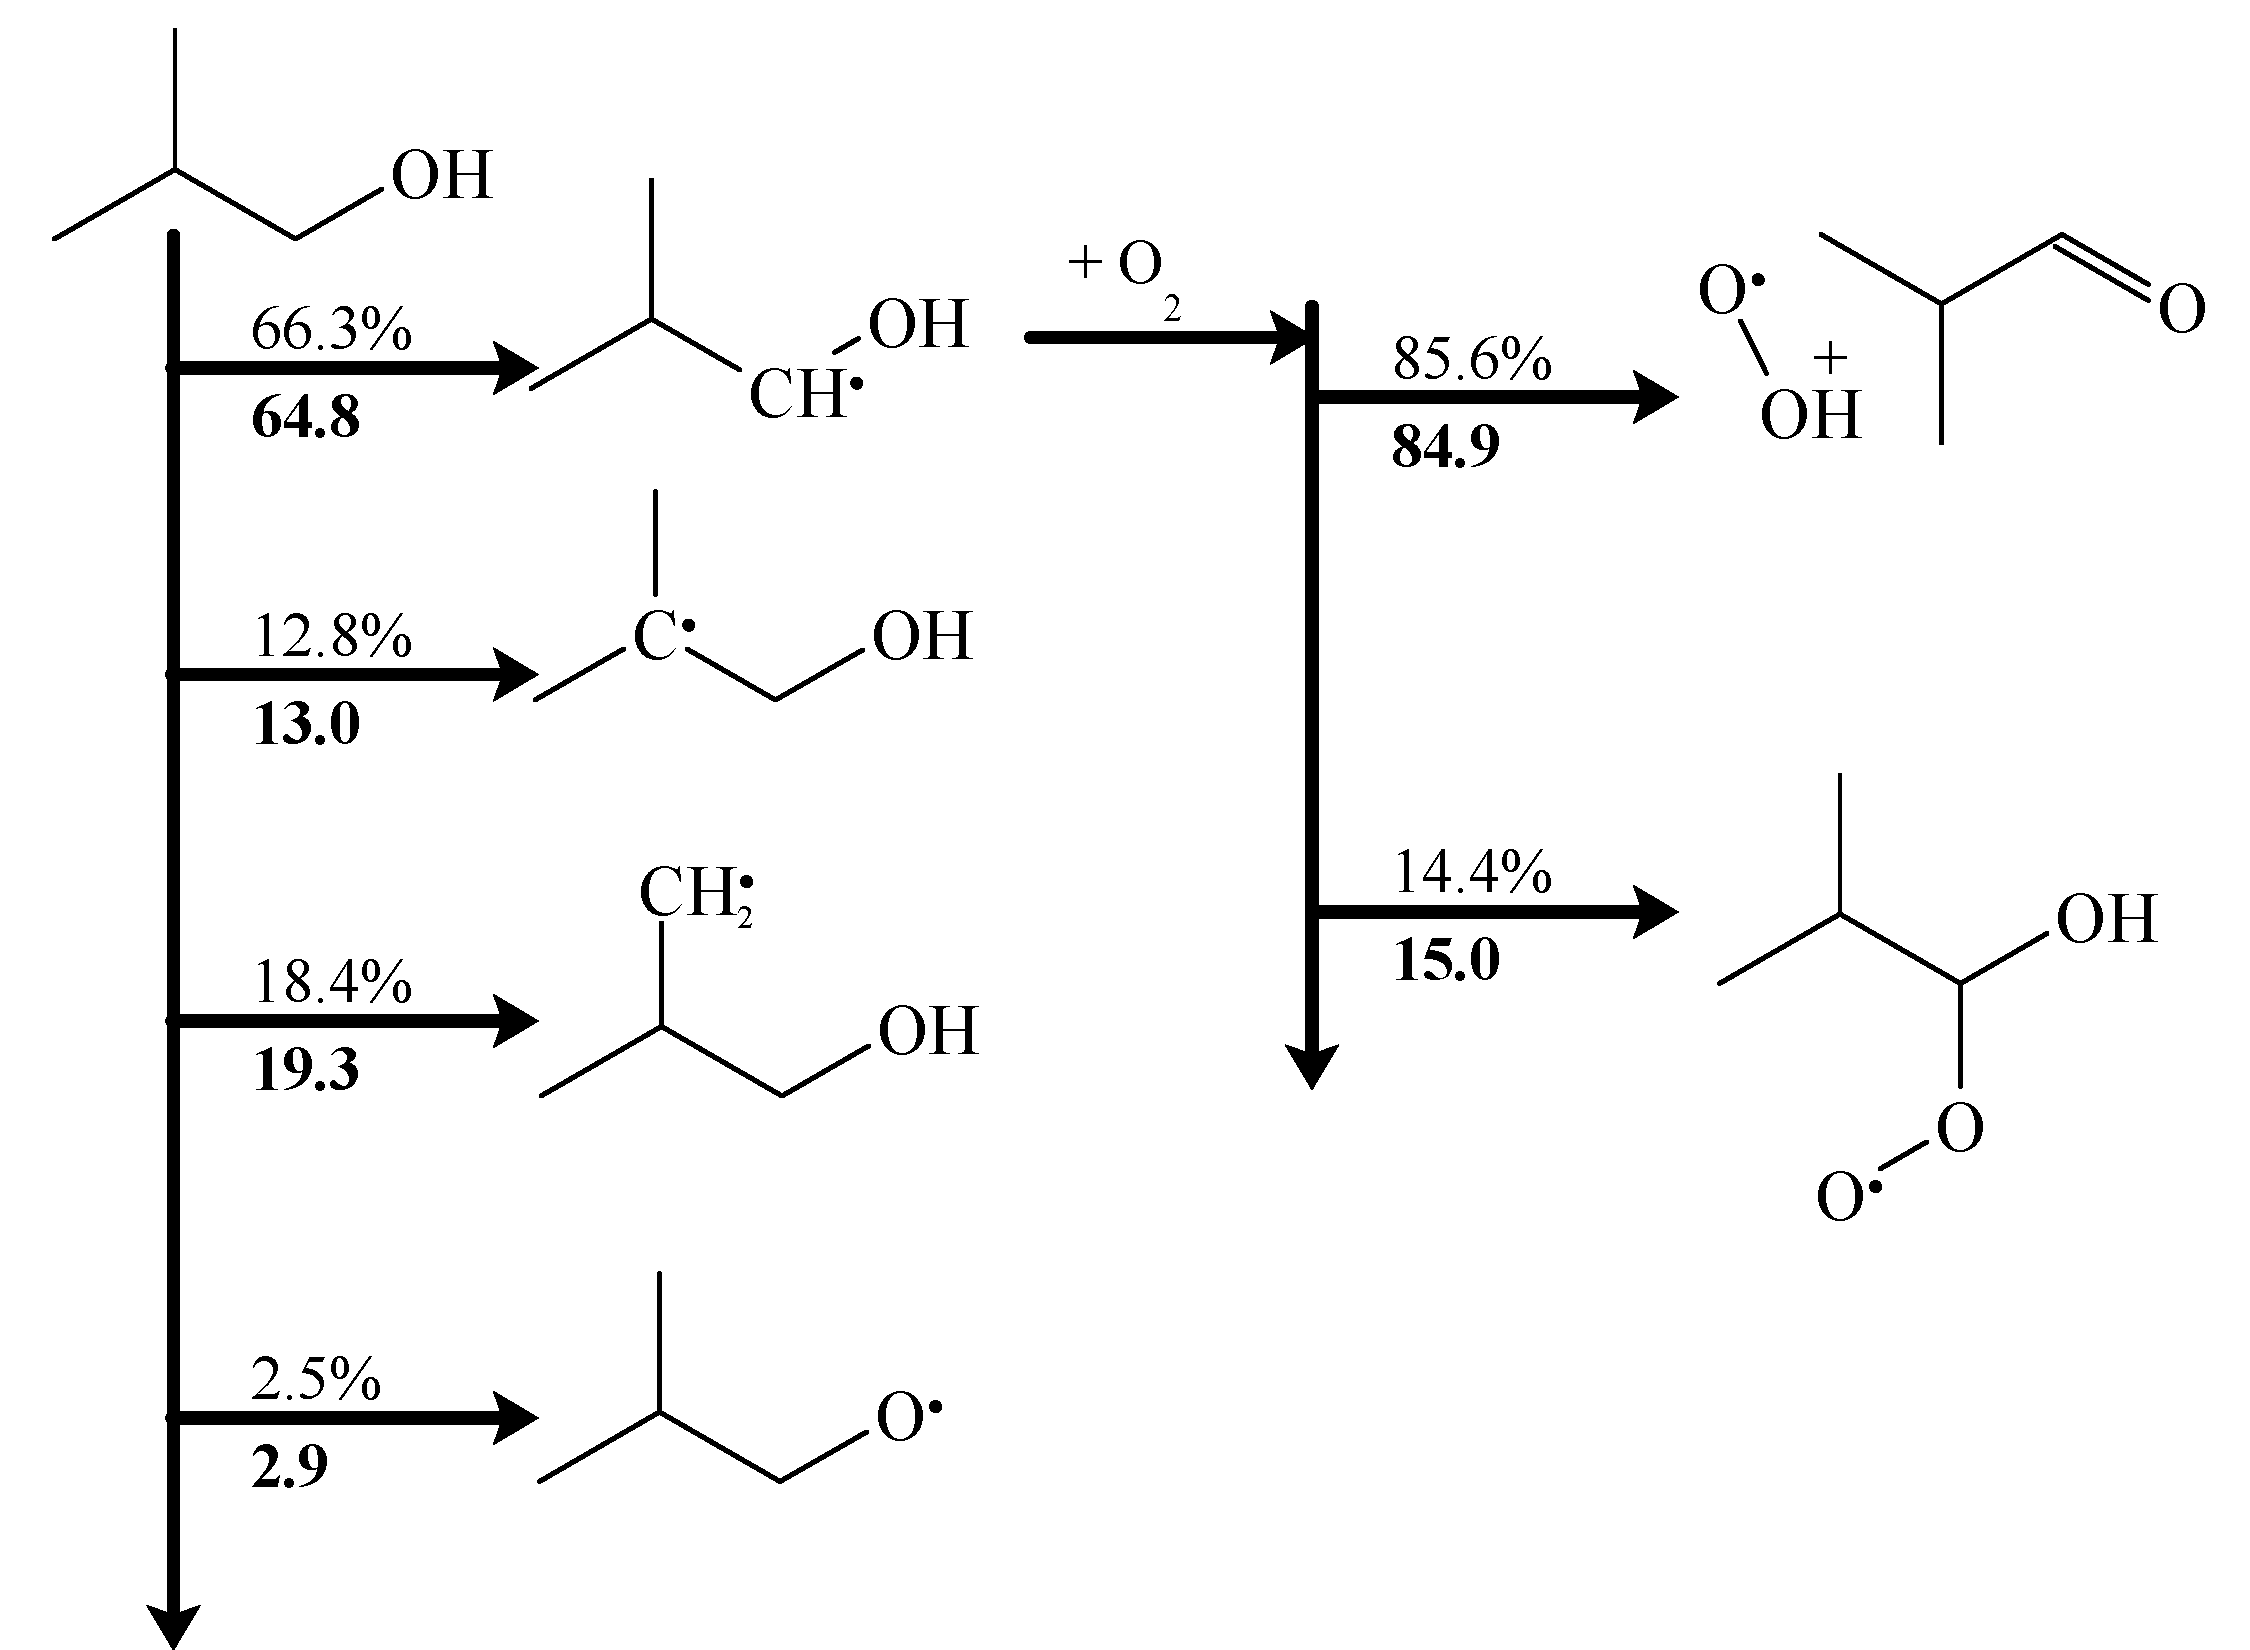
\includegraphics[width=7.9cm]{03-Butanol/buoh-ipath}}
        {\caption{Pathway analysis for simulations of \iBuOH{} at
            temperature of \SI{750}{\kelvin}, in stoichiometric air, using the mechanism of
            \textcite{Sarathy2012}. Percentages in normal text represent an
            initial condition of \SI{15}{\bar}; bold text is for \SI{30}{\bar}.}
        \label{fig:buoh-ipath}}
    \end{floatrow}
\end{figure}

In the following discussion, carbon-centered radicals are labeled according to
their distance from the hydroxyl moiety in the fuel molecule, as shown in
\cref{fig:buoh-isomers}. As expected at the relatively low temperature of this analysis, H-abstraction
reactions dominate over unimolecular decomposition for all four isomers. It is
also expected that \textit{n}-, \textit{s}-, and \iBuOH{} react
primarily to their respective $\alpha$-hydroxybutyl radicals, since the
$\alpha$ C-H bond has the lowest energy \cite{Sarathy2012}. Due to its unique
structure, \tBuOH{} does not have an $\alpha$-hydroxybutyl radical
that can be formed by H-abstraction, so \tBuOH{} is primarily
consumed to form the $\beta$-hydroxybutyl radical, because the O-H bond energy
is much higher than $\beta$ C-H bond energies.

The unique structure of \tBuOH{} continues to affect the second level
of reactions. In the temperature and pressure regime investigated,
\tBuOH{} tends to add to molecular oxygen at the carbon radical site,
forming a hydroxybutylperoxy (RO$_2$) species. That this pathway is dominant is
due to the fact that \tBuOH{} has no $\alpha$-hydroxybutyl radical.
For the other three butanol isomers that do have an $\alpha$-hydroxybutyl
radical, the second level of reactions primarily produces an aldehyde + HO$_2$
by direct reaction–--no hydroxybutylperoxy adduct is formed in this reaction,
and there is no possibility for typical hydrocarbon low-temperature chain
branching. Therefore, it is hypothesized that the pre-ignition heat release
seen in \tBuOH{} is caused by the oxygen addition to the fuel radical
to form $\beta$-hydroxybutylperoxy, which is an exothermic reaction.

\Cref{fig:buoh-heat} shows the total cumulative heat release of each isomer
and the cumulative heat release of an important reaction for each of the
isomers (inset), from a CONV simulation with initial conditions of \SI{750}{\kelvin} and
\SI{30}{\bar}; analysis of \SI{15}{\bar} results is substantially similar. The cumulative heat
release in the inset is found by integrating the heat release by each reaction
with respect to time, while the reactions shown are the respective reactions
that have released the most heat up to the 20\% fuel consumption point for each
isomer. The abscissa of the plot is the fuel conversion, in percent. This
choice of x-axis allows a fair comparison of the heat release, because the
ignition delays of each isomer are markedly different, so comparing the heat
release with a time axis is more difficult. In \cref{fig:buoh-heat},
exothermicity is represented by positive quantities.

In \cref{fig:buoh-heat}, it is clear that \tBuOH{} has higher
heat release at low fuel consumption (during the induction period) than the
other three isomers. In addition, the primary heat release reaction for
\tBuOH{} has created much more heat than the primary reactions of the
other three isomers. As the reactions proceed, and the temperature increases,
the reverse reaction in the \tBuOH{} case becomes more important, and
the heat release contribution of this oxygen-addition reaction levels off. The
dominance of this reaction at early times is unique to \tBuOH{}
ignition, and appears to be driving the pre-ignition heat release.

\begin{figure}
    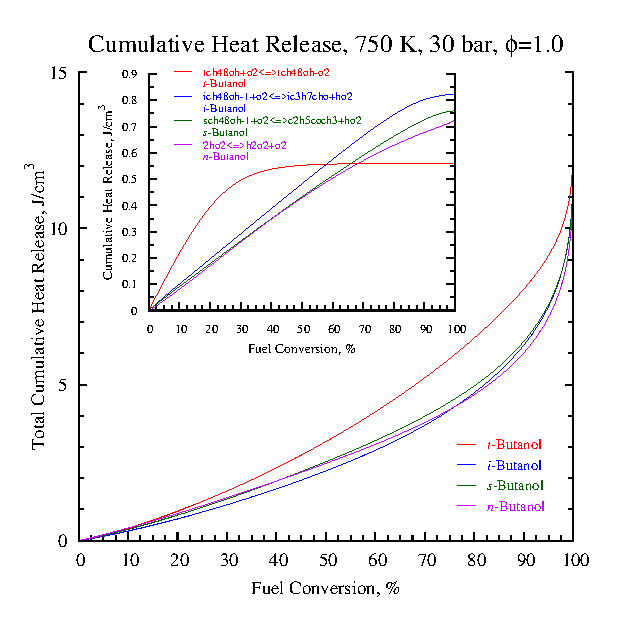
\includegraphics[height=11cm]{03-Butanol/buoh-heat}
    \caption{Total cumulative heat release and cumulative heat release by
        important reactions (inset) as a function of fuel consumption from a
        simulation using the mechanism of \textcite{Sarathy2012} with initial
        conditions of \SI{750}{\kelvin} and \SI{30}{\bar}, in stoichiometric air. See
        \cref{fig:buoh-reacs} for definitions of reactions in the inset.}
    \label{fig:buoh-heat}
\end{figure}

\begin{figure}
    R1: \quad \raisebox{-0.5\height}{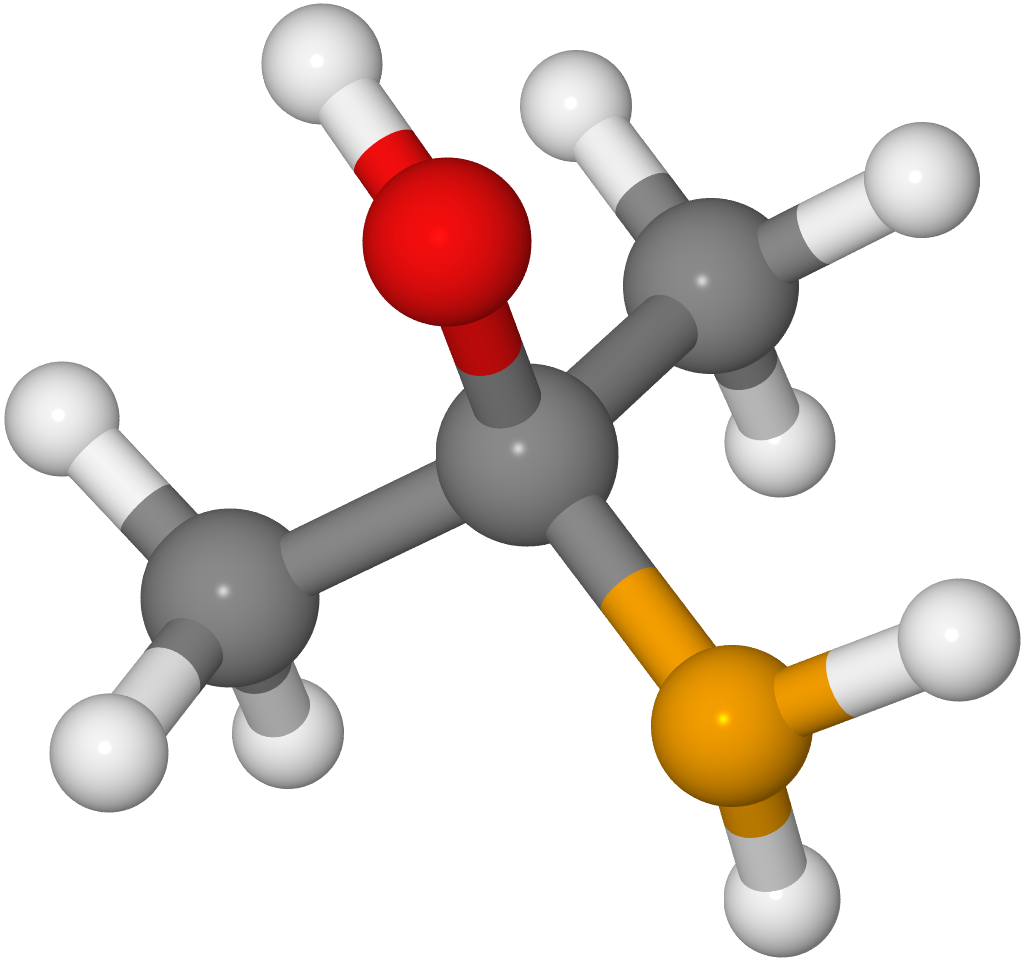
\includegraphics[height=2cm]{03-Butanol/buoh-reactions/tc4h8oh}}
    {\Large \textbf{+}}\enspace
    \raisebox{-0.5\height}{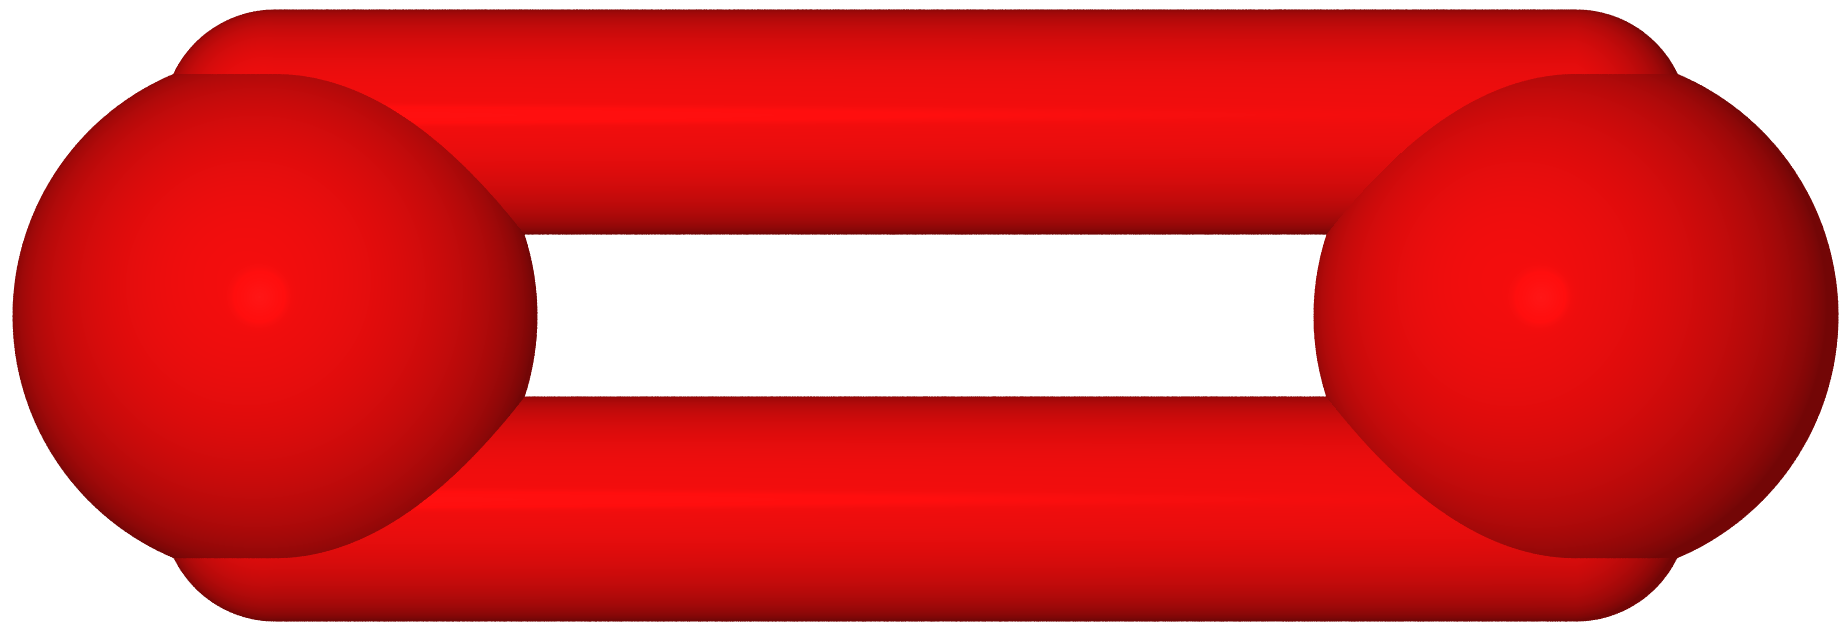
\includegraphics[height=0.5cm]{03-Butanol/buoh-reactions/oxygen}}
    {\Large \textbf{$\leftrightarrow$}}
    \raisebox{-0.5\height}{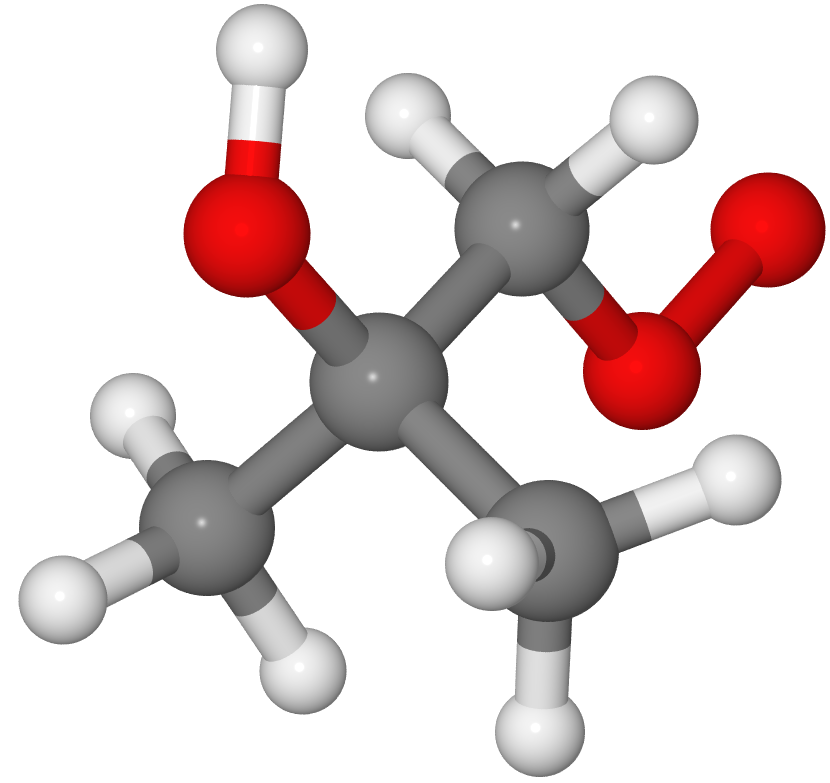
\includegraphics[height=2cm]{03-Butanol/buoh-reactions/t-hydroxybutylperoxy}}

    R2: \quad \raisebox{-0.5\height}{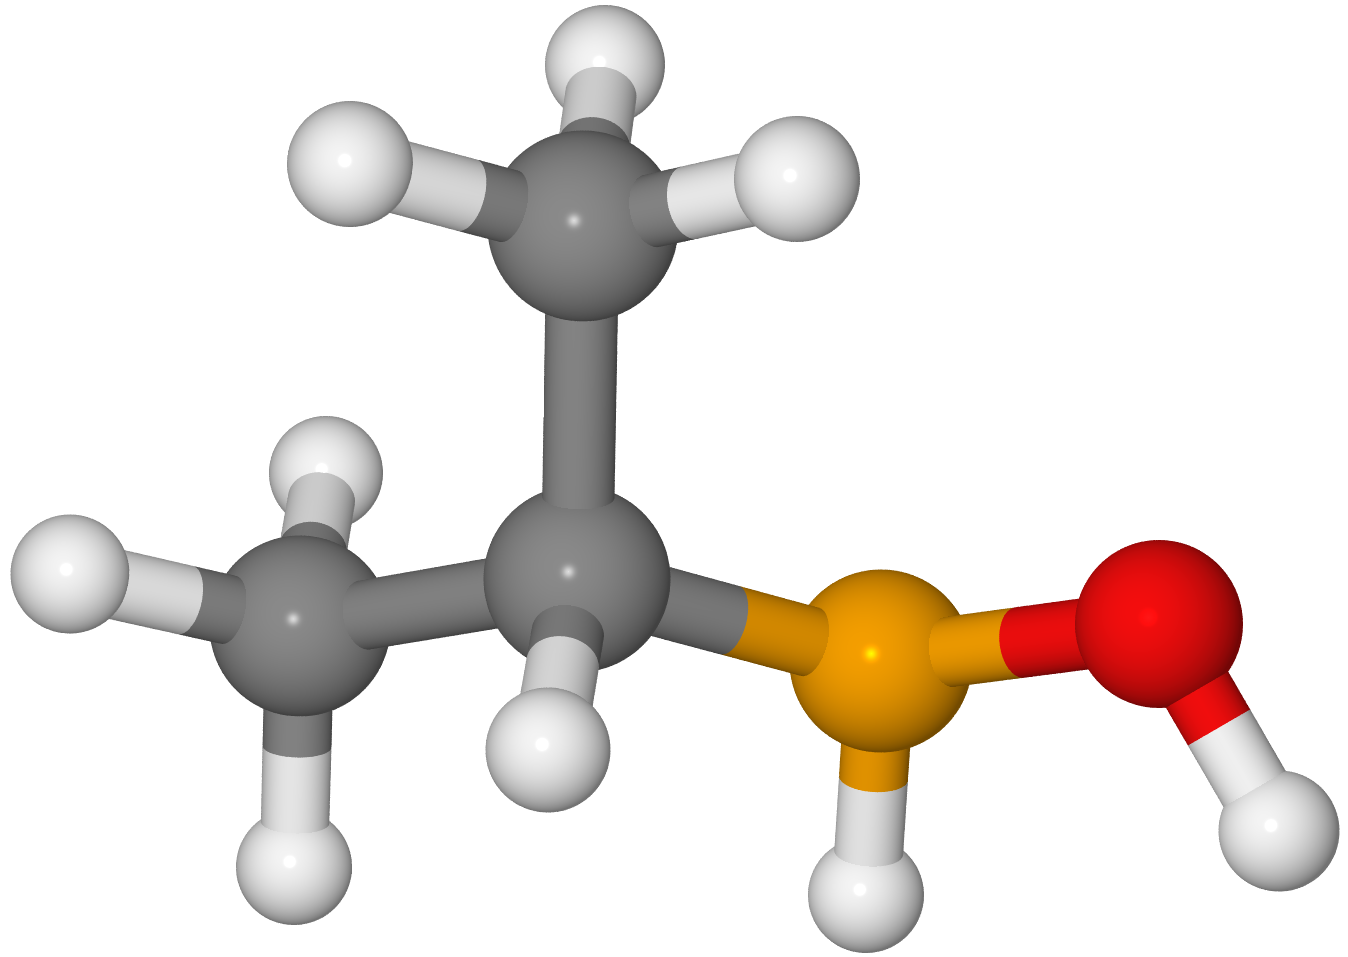
\includegraphics[height=2cm]{03-Butanol/buoh-reactions/ic4h8oh-1}}
    {\Large \textbf{+}}\enspace
    \raisebox{-0.5\height}{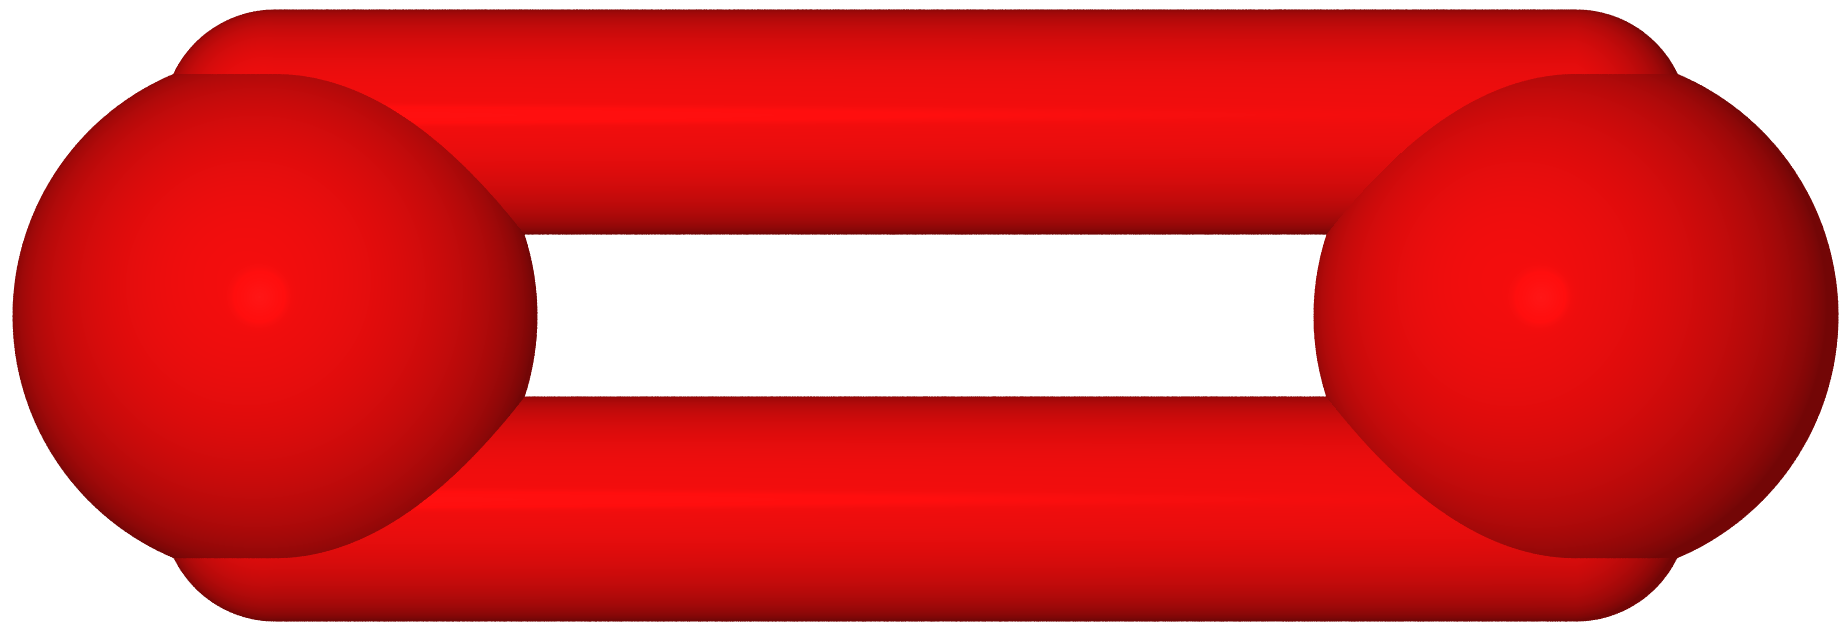
\includegraphics[height=0.5cm]{03-Butanol/buoh-reactions/oxygen}}
    \enspace{\Large \textbf{$\leftrightarrow$}}
    \raisebox{-0.5\height}{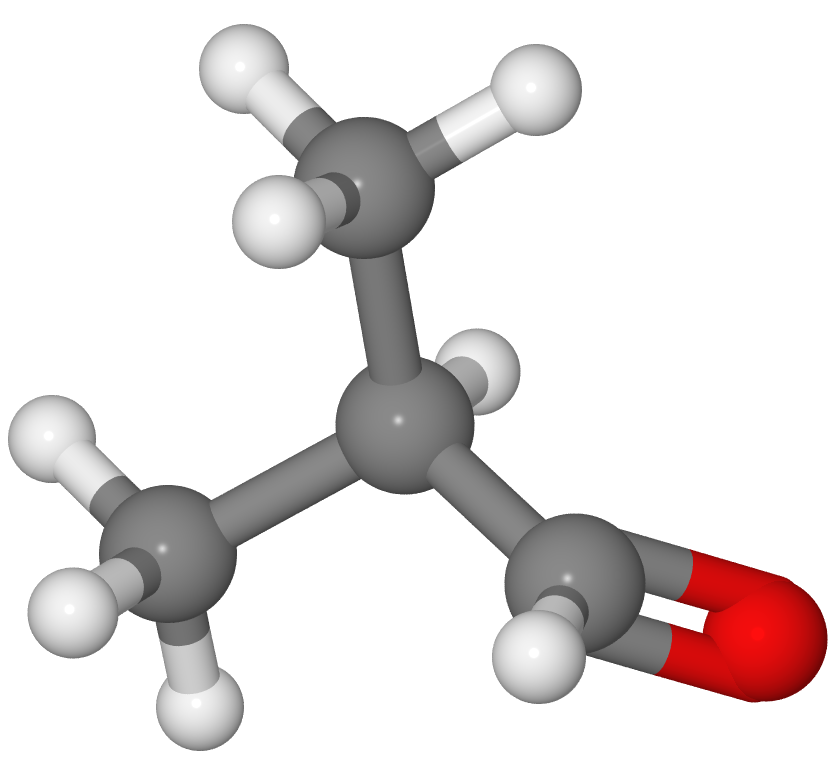
\includegraphics[height=2cm]{03-Butanol/buoh-reactions/iso-butanal}}
    {\Large \textbf{+}}\enspace
    \raisebox{-0.5\height}{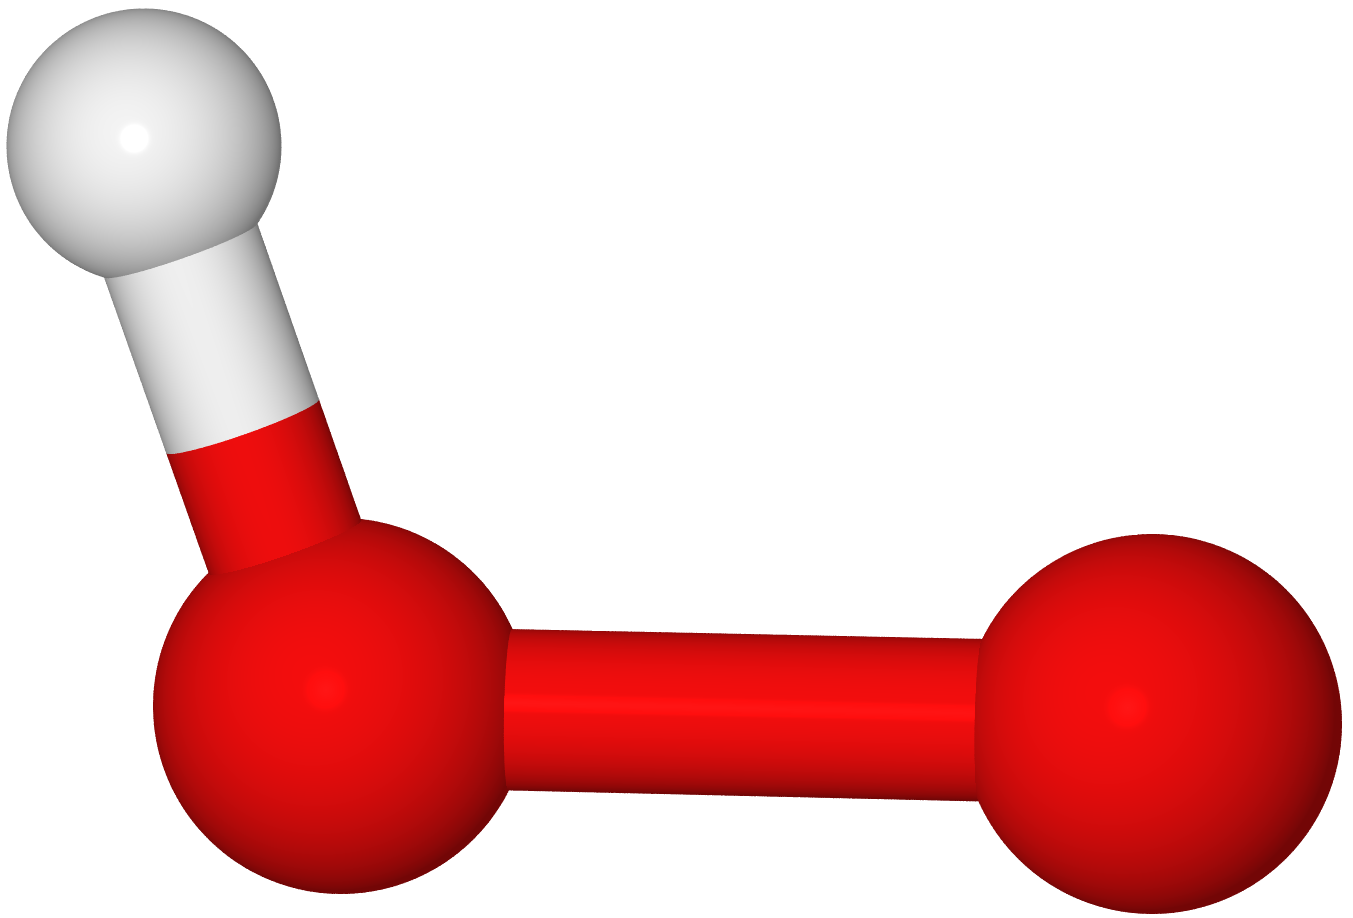
\includegraphics[height=1cm]{03-Butanol/buoh-reactions/hydroperoxy}}

    R3: \quad \raisebox{-0.5\height}{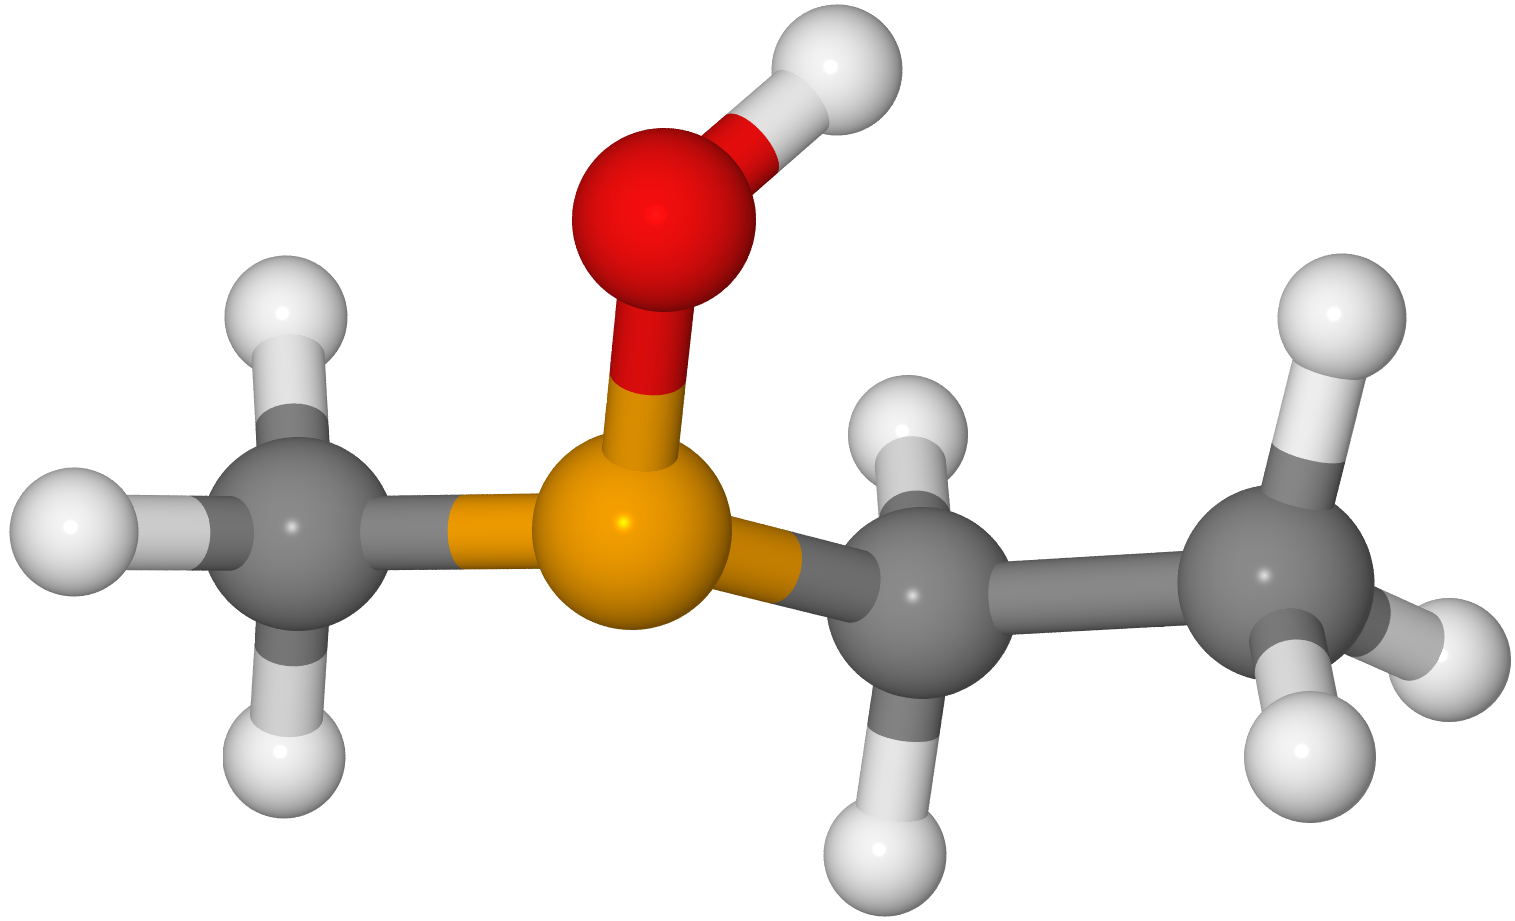
\includegraphics[height=2cm]{03-Butanol/buoh-reactions/sc4h8oh-1}}
    {\Large \textbf{+}}\enspace
    \raisebox{-0.5\height}{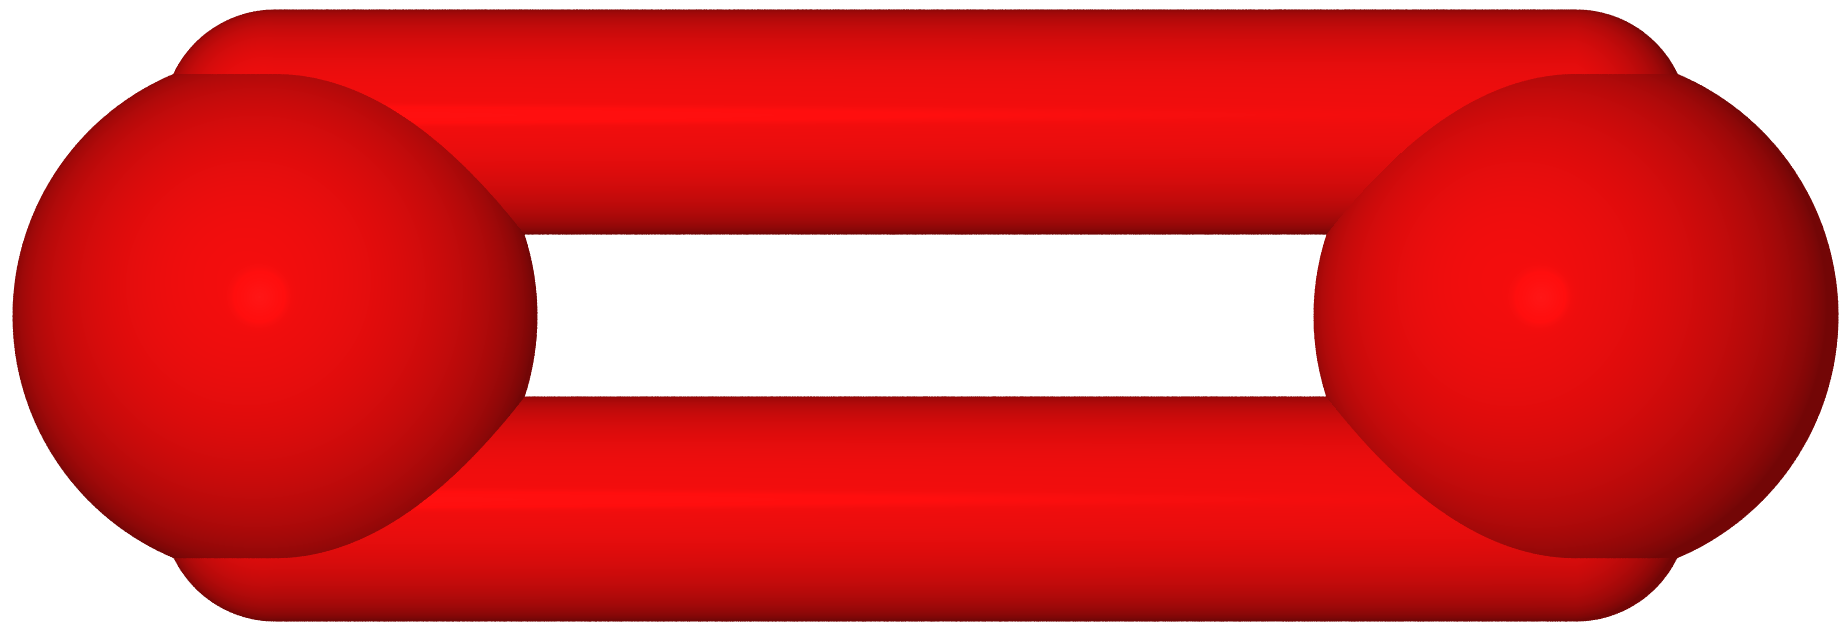
\includegraphics[height=0.5cm]{03-Butanol/buoh-reactions/oxygen}}
    \enspace{\Large \textbf{$\leftrightarrow$}}
    \raisebox{-0.5\height}{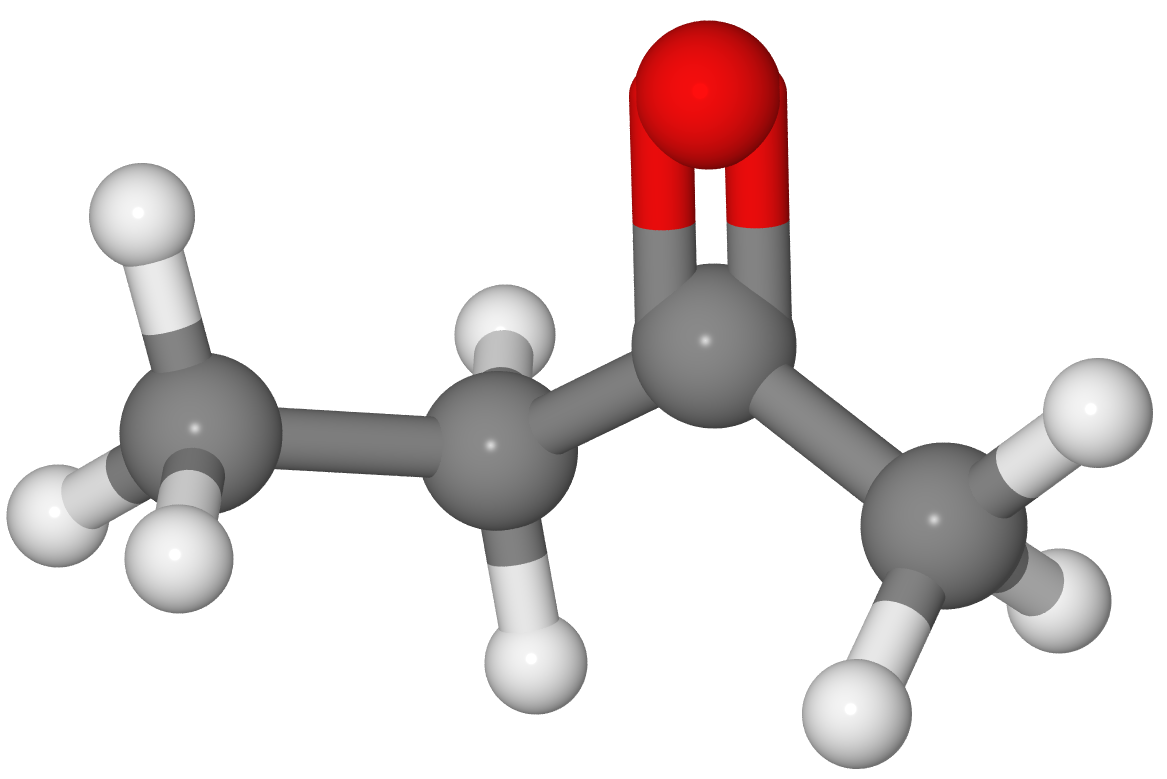
\includegraphics[height=2cm]{03-Butanol/buoh-reactions/2-butanal}}
    {\Large \textbf{+}}\enspace
    \raisebox{-0.5\height}{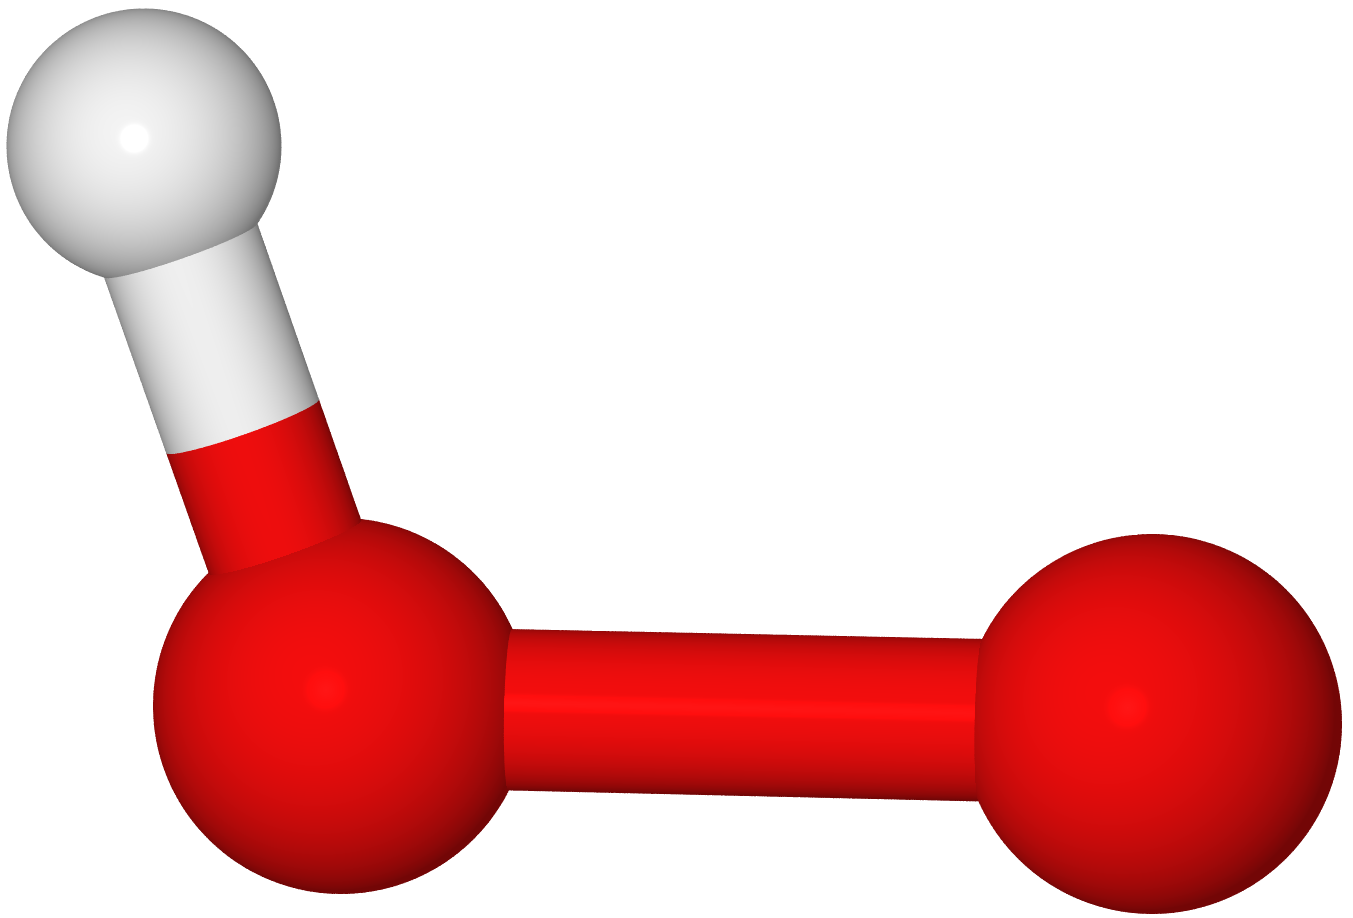
\includegraphics[height=1cm]{03-Butanol/buoh-reactions/hydroperoxy}}

    \blankline

    R4: \quad \raisebox{-0.5\height}{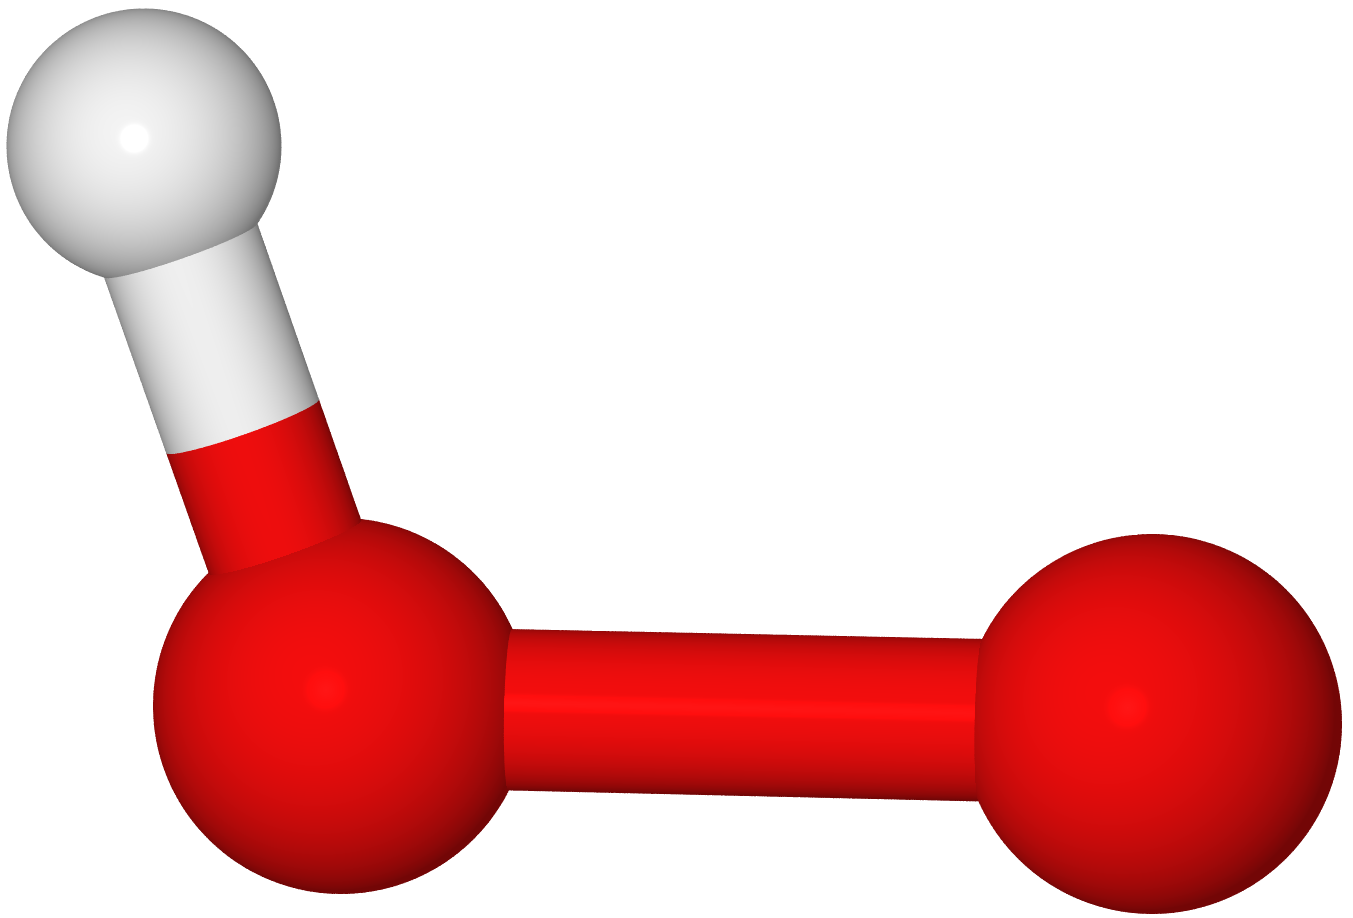
\includegraphics[height=1cm]{03-Butanol/buoh-reactions/hydroperoxy}}
    {\Large \textbf{+}}\enspace
    \raisebox{-0.5\height}{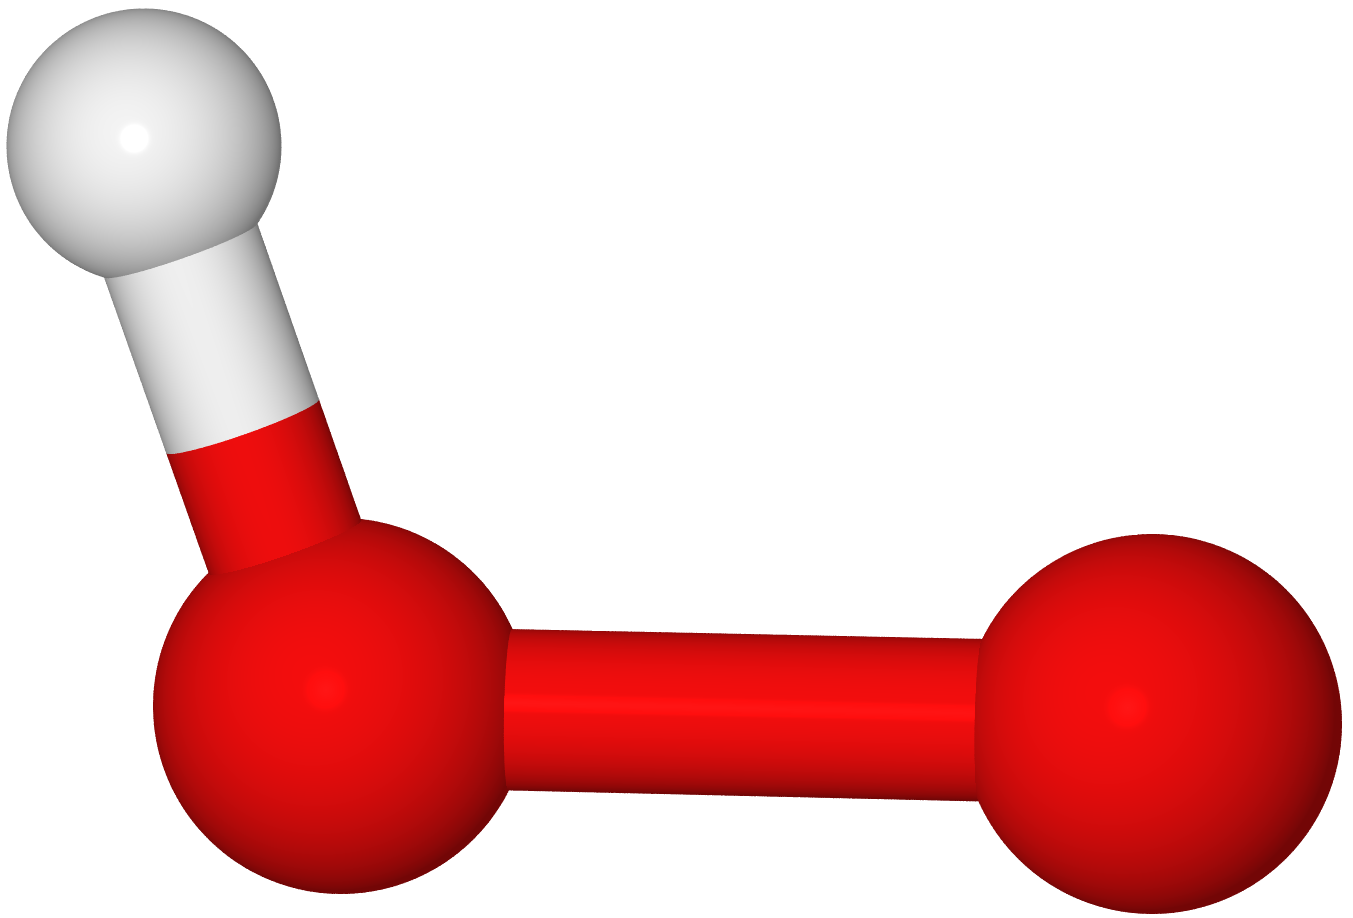
\includegraphics[height=1cm]{03-Butanol/buoh-reactions/hydroperoxy}}
    {\Large \textbf{$\leftrightarrow$}}\enspace
    \raisebox{-0.5\height}{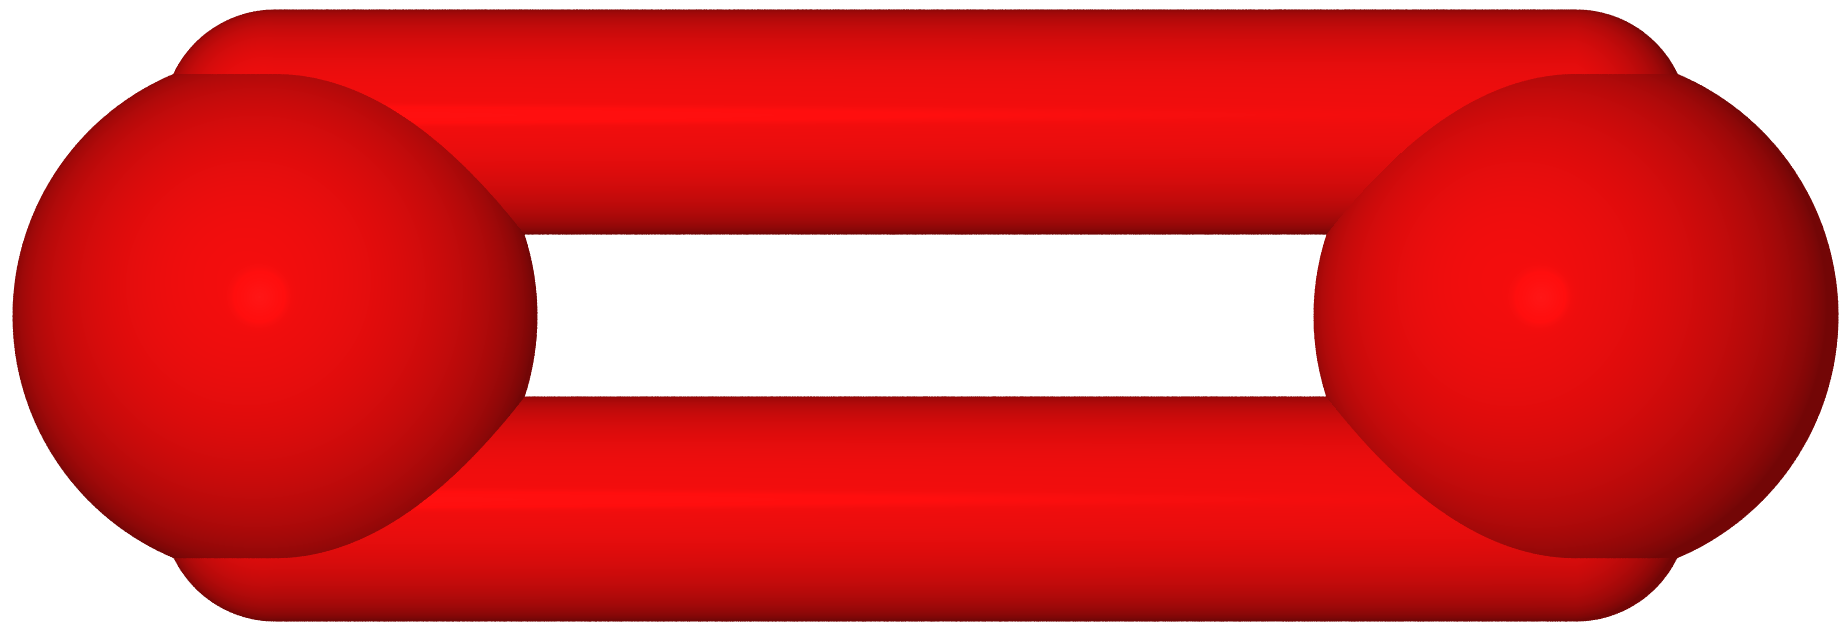
\includegraphics[height=0.5cm]{03-Butanol/buoh-reactions/oxygen}}
    \enspace{\Large \textbf{+}}\enspace
    \raisebox{-0.5\height}{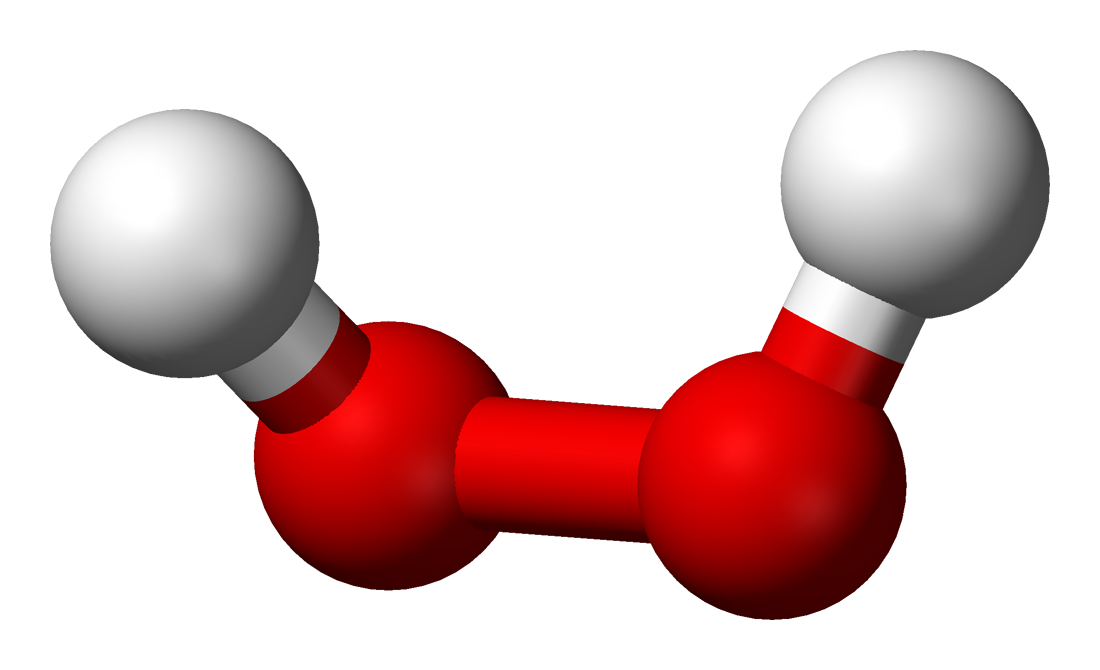
\includegraphics[height=1cm]{03-Butanol/buoh-reactions/hydrogen-peroxide}}

    \caption{Reactions causing the most heat release in the ignition of the
        butanol isomers. The reaction number refers to \cref{fig:buoh-heat}.}
    \label{fig:buoh-reacs}
\end{figure}

Other researchers have also undertaken studies of the low to intermediate
temperature combustion of \tBuOH{}. \textcite{Lefkowitz2012}
performed a study in the Variable Pressure Flow Reactor (VPFR) at Princeton
University on the oxidation of \tBuOH{} over the temperature range
from \SIrange{680}{950}{\kelvin}, at \SI{12.5}{atm} and stoichiometric mixture conditions. It is
interesting to note that they found no evidence of traditional hydrocarbon
low temperature chemistry. They did, however, find significant quantities of
acetone, peaking at approximately \SI{800}{\kelvin}. \textcite{Lefkowitz2012} concluded
that the primary pathways of acetone formation are tautomerization of
propen-2-ol and $\beta$-scission of the alkoxy radical, based on an analysis
of the mechanism from \textcite{Grana2010}. Both of these pathways are
dependent on unimolecular decomposition of the hydroxybutyl radicals. However,
this mechanism has only been validated for flame studies; indeed, an updated
version of this model (by \textcite{Frassoldati2012}) is unable to predict the
low-temperature ignition delays measured in this study and hence is not
considered for analysis.

In contrast to the study of \textcite{Lefkowitz2012} path analysis of the
mechanism by \textcite{Sarathy2012} shows that unimolecular decomposition
of the hydroxybutyl radicals is not the most important pathway; as mentioned
earlier, the most important pathway is the formation of
$\beta$-hydroxybutylperoxy. Further analysis shows that the primary pathway of
reaction of the \tBuOH{} $\beta$-hydroxybutylperoxy species is
through the Waddington mechanism. The Waddington mechanism has been shown
experimentally to be an important pathway for $\beta$-hydroxypentylperoxy
radicals in the low temperature combustion of \textit{i}-pentanol
\cite{Welz2012}, as well as the $\beta$-hydroxybutylperoxy radicals of
\textit{i}- and \tBuOH{} \cite{Welz2013b}. \textit{t}-Butanol only
produces $\beta$-hydroxybutyl radicals, and one of the products of the
Waddington pathway in \tBuOH{} is acetone (the others are
formaldehyde and hydroxyl radical); over 88\% of the acetone produced up to the
20\% fuel consumption point is produced by the Waddington reaction. The study
in the VPFR thus provides further evidence of the importance of low-temperature
hydroxybutylperoxy chemistry in \tBuOH{}, although it is not
traditional hydrocarbon low-temperature chemistry.

Up to this point, the discussion has focused mainly on the importance of
hydroxybutylperoxy chemistry in \tBuOH{}. Nevertheless, the chemistry
of the hydroxybutylperoxy species is important in the combustion of the other
isomers of butanol as well. Using the high pressure ST at RWTH Aachen
University, \textcite{Vranckx2011} showed the importance of peroxy chemistry
pathways in the autoignition of \nBuOH{}. By adding a lumped peroxy
model to an existing kinetic model for \nBuOH{} combustion, they were
able to substantially improve agreement of the model with their experiments at
high pressure and low temperature. In their mechanism, \textcite{Sarathy2012}
included a semi-detailed peroxy chemistry model for all the isomers of butanol.
In fact, one of the main differences between the mechanism from
\textcite{Sarathy2012} and the MIT mechanism \cite{Hansen2013,Merchant2013} is
their respective treatment of the peroxy mechanism. Specifically,
oxygen-addition chemistry is not included in the MIT mechanism for
\iBuOH{} \cite{Hansen2013,Merchant2013}. In addition, the radical
that primarily controls \iBuOH{} decomposition is hydroxyl (OH) in
the mechanism of \textcite{Sarathy2012} (generated by the peroxy chemistry
sub-mechanism), but is hydroperoxyl (HO$_2$) in the MIT mechanism
\cite{Hansen2013,Merchant2013} (generated from the direct $\alpha$-hydroxybutyl
+ O$_2$=HO$_2$ + aldehyde formation pathway).

In their work, \textcite{Sarathy2012} used the reaction rates computed by
\textcite{DaSilva2009} for the hydroxyethyl system (i.e. ethanol as the parent
fuel) to determine the rate of direct reaction of $\alpha$-hydroxybutyl and
oxygen to form aldehyde and HO$_2$, and then set the rate of oxygen addition to
the $\alpha$-hydroxybutyl radical (to form $\alpha$-hydroxybutylperoxy) so that
the total rate was less than the collisional limit. The rates of oxygen
addition for the other radicals were prescribed depending on the type of carbon
(primary, secondary, or tertiary) based on studies of butane and
\textit{i}-octane \cite{Sarathy2012}. Based on the well-known importance of
hydroxyl in driving the reactivity of combustion systems, and the sources of
the estimates for the reaction rates of oxygen addition to hydroxybutyl (i.e.
the entry to the pathway that controls the rate of hydroxyl formation), it can
be hypothesized that the rates of hydroxybutylperoxy formation are
overestimated in the mechanism of \textcite{Sarathy2012}, as the simulated
results under-predict the experimental data of \iBuOH{}.

This hypothesis is supported by the results shown in \cref{fig:buoh-sens},
which shows the linear brute force sensitivity of the ignition delay ($\tau$)
of \iBuOH{} with respect to changes in the $\mathrm{A}$-factor of the rate coefficient, using
the mechanism from \textcite{Sarathy2012}. The percent sensitivity is defined
as the difference between the ignition delay when the $\mathrm{A}$-factor of each reaction
is halved and the nominal ignition delay, normalized by the nominal ignition
delay, as shown below:

\begin{equation}
    \label{eq:buoh-sens}
    S_i=\frac{\tau(0.5\mathrm{A}_i )-\tau(\mathrm{A}_i )}{\tau(\mathrm{A}_i)} \times 100\%
\end{equation}

Therefore, negative sensitivity means that halving the $\mathrm{A}$-factor of a reaction
decreases the ignition delay, and positive sensitivity indicates the ignition
delay increases. These results are for CONV simulations with initial conditions
of \SI{750}{\kelvin} and \SI{30}{\bar} as well as \SI{1200}{\kelvin} and \SI{30}{\bar}.

\begin{figure}
    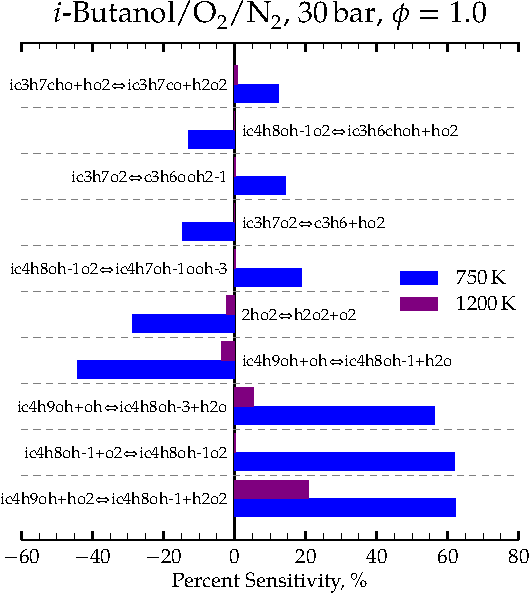
\includegraphics[width=10cm]{03-Butanol/buoh-sens}
    \caption{Linear brute force sensitivity analysis of the ignition delay with
        respect to the A-factors of the listed reactions in the mechanism from
        \textcite{Sarathy2012}. Positive quantities indicate the ignition delay
        is increased when the $\mathrm{A}$-factor is halved.}
    \label{fig:buoh-sens}
\end{figure}

The most sensitive reaction at the lower temperature is the initiation reaction
of the fuel with hydroperoxyl radical to form the primary fuel radical and the
second most sensitive reaction is the addition of oxygen to the primary
radical. Both of these reactions have positive sensitivities, indicating that
reducing the rate of these reactions increases the ignition delay
and improves the agreement of the simulations relative to the experiments
in this case. It is apparent, then, that reducing the amount of fuel
propagating into the low temperature chain branching pathway of oxygen
addition to the primary $\alpha$-radical improves the simulated results.
Interestingly, the \iBuOH{} system is not sensitive to the rates of
oxygen addition to the hydroxybutyl radicals other than the
$\alpha$-radical. At the higher temperature of \SI{1200}{\kelvin}, there
is little sensitivity on the ignition delay by changing the rate of the
oxygen-addition reaction, demonstrating its lack of influence at higher
temperatures.

As a final comparison, we have modified this pathway in the mechanism from
\textcite{Sarathy2012} so that the rate of oxygen addition to the primary
fuel radical is arbitrarily set to zero; that is, the rate of the reaction
ic4h8oh-1+o2=ic4h8oh-1o2 is set to zero by zeroing the $\mathrm{A}$-factor, while the
rates of the other oxygen addition reactions were unchanged. This unphysical
situation substantially changes the results of simulations for
\iBuOH{} --- removing this pathway in the mechanism from
\textcite{Sarathy2012} brings the simulations into close agreement with the
ignition delay results from the MIT mechanism \cite{Hansen2013,Merchant2013},
which does not consider this reaction for \iBuOH{}. Since the other
oxygen addition reactions were unchanged, it is apparent that the addition of
oxygen to $\alpha$-hydroxybutyl is one of the controlling reactions for the
high-pressure, low-temperature ignition of \iBuOH{} using the
mechanism of \textcite{Sarathy2012}. It is therefore concluded that a detailed
examination of the rates of direct formation of aldehyde+HO$_2$ and oxygen
addition to the $\alpha$-hydroxybutyl radical are required to better predict
the low-temperature ignition behavior of \iBuOH{}. Furthermore, based
on the other results of this study, a detailed analysis of the oxygen addition
reactions to all the isomers of butanol is probably warranted.

\section{Conclusions}
\label{sec:buoh-conclusions}

In this work, ignition delays for all four isomers of butanol in stoichiometric
mixture with air have been presented over the low to intermediate temperature
range, and at two compressed pressures of \SIlist{15;30}{\bar}. The order of
reactivity of the isomers is \nBuOH{}$>$\sBuOH{}$\approx$\iBuOH{}$>$\tBuOH{}
at the lower pressure, but changes to \nBuOH{}$>$\tBuOH{}$>$\sBuOH{}$>$\iBuOH{}
at the higher pressure. This unexpected result is partially explained by
the fact that there is substantial pre-ignition heat release present
for \tBuOH{}. To help understand the nature of the pre-ignition heat
release of \tBuOH{}, studies at off-stoichiometric conditions,
$\phi=\num{0.5}$ and $\phi=\num{2.0}$ in air, are also conducted.

Comparisons of the experimentally measured ignition delays with two kinetic
mechanisms show good agreement for certain isomers, but relatively poorer
agreement for others. The kinetic mechanism of \textcite{Sarathy2012} is used
to further elucidate the chemical processes controlling the autoignition of
these butanol isomers. Pathway analysis of the fuel decomposition shows that
\textit{n}-, \textit{s}-, and \iBuOH{} primarily form
$\alpha$-hydroxybutyl radicals, because the proximity of the $\alpha$ carbon to
the hydroxyl group reduces the C-H bond energy. The $\alpha$-hydroxybutyl radicals
tend to form an aldehyde plus HO$_2$  directly, without forming a
hydroxybutylperoxy complex. However, due to its unique structure,
\tBuOH{} can only form $\beta$-radicals; these radicals do not have
the tendency to react with oxygen to directly form HO$_2$  and an aldehyde.
Rather, \tBuOH{} preferentially adds oxygen to the fuel radical site.
It is hypothesized that this reaction, O$_2$  addition to form
hydroxybutylperoxy, causes the pre-ignition heat release in \tBuOH{}
and leads to a chain propagation pathway through the Waddington mechanism. The
fact that this oxygen-addition reaction is preferred is unique to
\tBuOH{}, although a detailed understanding of the peroxy chemistry
of alcohols is still of vital importance to the other butanol isomers. This is
further demonstrated in this work for the case of \iBuOH{}, where the
ignition delay is quite sensitive to both the rate of primary fuel
radical formation and to the rate of oxygen addition to the primary fuel
radical. It is also noted that \nBuOH{} autoignition was
quite sensitive to peroxy chemistry in the study of \textcite{Vranckx2011}.

All together, these analyses show the importance of the peroxy chemistry
pathways in the autoignition of the butanols. Further experimental studies,
such as species profiles from the low temperature ignition of the butanol
isomers, could help reduce uncertainty in the pathways of fuel breakdown.
Finally, further understanding of the rates of the peroxy pathways is
important and therefore further theoretical and quantum chemical studies are
warranted.

\end{document}
